\documentclass[12pt]{article}
\usepackage[latin9]{inputenc}
\usepackage{microtype}
\usepackage[letterpaper]{geometry}
\geometry{verbose,tmargin=1in,bmargin=1in,lmargin=1in,rmargin=1in}
\pagestyle{plain}
\usepackage{color}
\usepackage{float}
\usepackage{amsmath}
\usepackage{amssymb}
\usepackage{graphicx}
\usepackage[authoryear]{natbib}
\usepackage{chngcntr}
\usepackage{subcaption}

%%%%%%%%%%%%%%%%%%%%%%%%%%%%%%  SPACING
\usepackage{setspace}

\onehalfspacing % working paper spacing

%\doublespacing % journal submission spacing
%\usepackage{footmisc} % journal submission spacing
%\renewcommand{\footnotelayout}{\doublespacing} % journal submission spacing
%%%%%%%%%%%%%%%%%%%%%%%%%%%%%% 

\usepackage{xr}
%\usepackage{xr-hyper}
\externaldocument{AGS_Output_Subsidies_Online_Appendices}

\usepackage[unicode=true,
 bookmarks=false,
 breaklinks=false,pdfborder={0 0 1},backref=false,
 hidelinks]
 {hyperref}
\usepackage{breakurl}

\makeatletter

%%%%%%%%%%%%%%%%%%%%%%%%%%%%%%  PACKAGES FOR COMMENTING
% USER WRITTEN COMMENT COMMAND

% IF SELECTED, COMMAND WILL NOT DISPLAY COMMENTED TEXT  
%\newcommand{\comment}[1]{}  %comment not shown

%IF SELECTED, COMMAND WILL PRINT COMMENTED TEXT IN BLUE  
\newcommand{\comment}[1]
{{\bfseries \color{red} #1}} %comment shown

%%%%%%%%%%%%%%%%%%%%%%%%%%%%%% User specified LaTeX commands.
\setcounter{MaxMatrixCols}{10}

\usepackage{booktabs}% Pretty tables
\usepackage{tabularx}% 
\usepackage{threeparttable}% For Notes below table

\usepackage{amsfonts}
\usepackage{multicol}
\usepackage{lscape}
\usepackage{rotating}

\usepackage{changepage}
\usepackage{pdfpages}
\usepackage{geometry}
\usepackage{graphicx}

\usepackage{xcolor}


%PUT DATE IN MONTH-YEAR
\usepackage{datetime}
\newdateformat{monthyeardate}{%
  \monthname[\THEMONTH] \THEYEAR}
\makeatother

\begin{document}

\title{Investment versus Output Subsidies: Implications of Alternative Incentives for Wind Energy}

\author{Joseph E. Aldy, Todd D. Gerarden, and Richard L. Sweeney\thanks{Aldy: Harvard Kennedy School, Resources for the Future, National Bureau of Economic Research, and Center for Strategic and International Studies (email: \href{mailto:joseph_aldy@hks.harvard.edu}{joseph\_{}aldy@hks.harvard.edu}); Gerarden: Cornell University (email: \href{mailto:gerarden@cornell.edu}{gerarden@cornell.edu}); Sweeney: Boston College (email: \href{mailto:sweeneri@bc.edu}{sweeneri@bc.edu}). Data and code for replication are available at \href{https://github.com/rlsweeney/public_ags_output_subsidies}{https://github.com/rlsweeney/public\_ags\_output\_subsidies}. Blake Barr, Juliet Bramante, Jeff Bryant, Napat Jatusripitak, Ken Norris, Michael O'Brien, Carlos Paez, Jun Shepard, Avi Zevin, and Howard Zhang provided excellent research assistance. Thanks to Scott Walker, Gabe Chan and Joern Huenteler for assistance with wind speed data; and Curtis Carlson, John Horowitz, and Adam Looney for assistance with historical tax policy information. This project has been supported by the Alfred P. Sloan Foundation (grant 2015-13862) and the Harvard University Center for the Environment. Aldy acknowledges support from BP, the Taubman Center, and the Belfer Center. Gerarden acknowledges support from U.S. EPA STAR Fellowship no. FP-91769401-0. We have benefited from feedback provided at several conferences and seminars, as well as conversations with Alberto Abadie, Lucas Davis, Kelsey Jack, Jud Jaffe, Ken Gillingham, Justin Kirkpatrick, Joel Landry, Jeff Liebman, Erin Mansur, Paul Goldsmith-Pinkham, Matt Rogers, Dick Schmalensee, Jim Stock, and Martin Weitzman.}}


\date{\monthyeardate\today}
\maketitle
\begin{abstract}
\noindent This paper examines the choice between subsidizing investment and subsidizing output to promote socially desirable production. We exploit a natural experiment to estimate the impact of subsidy margin on the productivity of wind farms. Using instrumental variable and matching estimators, we find that investment subsidy claimants produce 10 \unskip to 12percent less power than they would have under the output subsidy. Accounting for extensive margin effects, we show that output subsidies are more cost-effective than investment subsidies over a large range of output targets. 

\vspace{1cm}

\noindent Keywords: tax credits, energy subsidies, instrument choice

\noindent JEL Codes: H23, Q42, Q48

\vspace{1cm}
\end{abstract}

\pagebreak
\section{Introduction}

Governments subsidize investment for a variety of reasons. When economic output falls well below potential output, policymakers subsidize investment to stimulate the economy. To address the market failure of innovation spillovers, governments subsidize research and development spending. To increase the supply of affordable housing, governments subsidize low-income housing development. To spur the replacement of pollution-intensive facilities, policymakers subsidize the construction of low-emission power plants. In each of these examples, the social benefits of subsidized investments are tied to the eventual \textit{output} they produce, not just the investment itself. Given this, it is noteworthy that governments also often \textit{directly} subsidize output in each of these settings, through government procurement, research prizes, housing vouchers, and tax credits for clean energy production. 

Is it better to subsidize investment or output? If the government's objective is to minimize the public expenditure necessary to meet an output target, the answer is theoretically ambiguous. Whether investment subsidies are more or less cost-effective than output subsidies depends on how intensively investment goods are used on the margin, compared to on average, and how substitutable they are with other unsubsidized inputs \citep{parish_relative_1982}. Despite the ubiquity of both types of subsidies, there is little empirical evidence comparing their cost-effectiveness in practice. 

In this paper, we provide the first direct empirical evidence on this topic. We focus on the U.S. wind power industry, where a unique policy innovation introduced through the American Recovery and Reinvestment Act of 2009 temporarily allowed project developers to choose between investment and output subsidies. Before January 1, 2009, wind farm developers could only claim the Production Tax Credit (PTC), equal to \$23 per megawatt-hour (MWh) for the first ten years of output. From 2009 to 2012, developers could choose between the PTC and the Section 1603 grant, an upfront cash payment equal to 30 percent of investment costs. We leverage this natural experiment to compare the relative cost-effectiveness of these investment and output subsidies using three sets of complementary analyses. 

First, we focus on the intensive margin and find that plants claiming the investment subsidy were 10 \unskip to 12percent less productive than they would have been under the output subsidy. These estimates reflect two empirical strategies that rely on different identifying assumptions. Since there is no within-plant variation in subsidy type, we compare the output of plants that selected the investment subsidy with those that selected the output subsidy. As one approach to address concerns about this selection, we restrict the sample to wind farms placed into service within 12 months of the January 1, 2009 policy change. Within this window, the long lead time of wind farm development ensures that all siting and capital decisions would have been fixed well before the 1603 program was even conceived. To estimate the effect of replacing output with investment subsidies, we instrument for investment subsidy selection with an indicator for whether a plant was eligible for the 1603 grant. For our second approach, we use a matched difference-in-differences estimator on the full population of wind farms placed into service between 2005 and 2012. We employ matching to identify those plants in the pre-2009 period that would have selected the investment subsidy had the 1603 grant been available. We then compare output between plants that, based on observables, appear to prefer output subsidies to those that appear to prefer investment subsidies before and after investment subsidies were made available.

Second, we evaluate the extensive margin gains associated with the introduction of the 1603 grant program and assess whether they could offset these intensive margin production losses. Long project lead times coupled with the short duration of the program limited the set of potential entrants to projects already in the development process when Congress unexpectedly legislated the program. Using more than a decade of data on wind farm proposals, we find little change in the probability that a proposed plant comes to fruition during the 1603 grant program period. In order to estimate how many proposed wind farms were ``saved'' by the grant program following the financial crisis, we use plant-specific investment cost and marginal revenue data to construct each plant's expected discounted lifetime profits, and find that only three \unskip percent of the 1603 recipients appear marginal to the investment subsidy. Accounting for both intensive and extensive margin impacts, we estimate that the 1603 program reduced total wind output among recipients by 4 \unskip percent, while \emph{increasing} the total public cost by 3 \unskip percent, relative to a counterfactual scenario in which all wind farms had received the PTC.

Third, we use these analyses to generate commensurable estimates of the public expenditure required to achieve a given quantitative renewable energy target under each regime. This allows us to make direct comparisons of investment and output subsidies over a large range of output targets. We show that, even if the intensive margin effect of output subsidies on plant productivity is ignored, output subsidies are more cost-effective than investment subsidies over a wide range of public output targets. This is due to a negative correlation between plant productivity and output price. Once we incorporate the estimated impact of output subsidies on plant productivity, output subsidies appear significantly cheaper. For example, over the entire population of wind farms entering from 2009 to 2012, we find that the same amount of wind power produced by a 30 percent investment subsidy could be achieved at $29$ percent lower cost using an output subsidy. 

Although this paper is primarily focused on subsidy cost-effectiveness, we also discuss the welfare implications of our results. As we explain in Section \ref{subsec:outputModel}, one way that output subsidies could increase wind farm productivity is by encouraging firms to exert more effort on operations and maintenance. However, output subsidies could also increase the quantity of wind power demanded, conditional on effort, by moving wind up in the electricity dispatch curve. We correlate monthly output with the frequency of negative prices to infer that this ``dispatch effect'' could explain between one-third and two-thirds of the estimated increase in plant productivity under output subsidies. Nevertheless, after reviewing evidence from the literature on emissions displaced by wind energy, we conclude that this decomposition is not essential for signing net benefits. Output subsidies appear preferable to investment subsidies in this setting, regardless of the mechanism through which they increase output.

Despite extensive research on both optimal taxation and instrument choice, there is little research on the relative performance of input and output subsidies.\footnote{The question was qualitatively discussed in several contexts in the 1980s. For example, \cite{stiglizWB1987} compares and contrasts crop price supports and fertilizer subsidies. \citet{schmalensee_appropriate_1980} considers the conceptual merits of government policy to increase energy production generally, and concludes that input subsidies build in ``potentially huge inefficiencies'' relative to an output subsidy.} There is a large literature on the effects of investment tax incentives across industries \citep[e.g.,][]{goolsbee_investment_1998,goolsbee_taxes_2004,house_temporary_2008}, but these papers do not compare investment incentives to alternative instruments that target output. A few relevant papers estimate dynamic structural models of \textit{adoption} in the solar industry \citep{burr2016subsidies,de_groote_subsidies_2019} or ethanol plant entry \citep{yi2018dynamic} in the presence of one of the two subsidies, and assess the impact of the other subsidy using counterfactual simulations. In contrast, we observe firms exposed to both types of subsidy simultaneously in the data, and exploit a natural experiment to directly compare outcomes across them. 

This paper also contributes to a growing literature on renewable energy policy. Several papers focus on estimating the environmental benefits of renewable electricity generation \citep[e.g.,][]{cullen_measuring_2013,novan_valuing_2015,callaway_location_2018,fell_emissions_2021}. While we are primarily concerned with cost-effectiveness, we discuss the efficiency implications of different subsidy margins in Section \ref{sec:Mechanism}. \citet{metcalf_investment_2010} relates the PTC to the user cost of capital and finds that wind investment is highly responsive to changes in tax policy. \citet{schmalensee_evaluating_2012} compares U.S. renewable subsidies to policy alternatives such as a feed-in tariff or a cap-and-trade program to limit emissions. Our paper is the first to study the impact of the incentives created by renewable subsidies on firm productivity. As such, we build upon prior work that showed electricity restructuring incentivized fossil fuel and nuclear power plants to operate more efficiently \citep[e.g.,][]{fabrizio_markets_2007,davis_deregulation_2012,cicala_when_2015}. \citet{petersen2021Spain} study the effect of output subsidies at high levels of renewable energy penetration, and find that switching to capacity-based payments for existing wind farms in Spain increased welfare by avoiding inefficient production on high wind days. In contrast, we compare output subsidies to investment subsidies in a setting where the policies affected firms on both the intensive and extensive margins, but where wind penetration levels were still relatively small. 

Finally, \cite{johnston_nonrefundable_2019} also studies the 1603 grant program. \citeauthor{johnston_nonrefundable_2019} focuses on the non-fungibility of the PTC and asks whether replacing it with a refundable tax credit or grant would increase wind power investment. Leveraging an identification approach similar to our IV strategy, \citeauthor{johnston_nonrefundable_2019} finds that wind farm developers value each PTC dollar at \$0.85. Crucially, the estimation approach used in that paper assumes the difference in marginal incentives between the PTC and 1603 grant has no impact on wind farm productivity. In contrast, we estimate the impact of these marginal incentives and find that they are large.

The rest of this paper proceeds as follows. Section~\ref{sec: Background} provides a brief introduction to the economics of wind energy, a summary of the policy environment, and a discussion of how production incentives differ under investment and output subsidies. Section~\ref{sec:Data} describes the data. Section~\ref{sec:Empirical-Strategy} summarizes the empirical strategy and results for our intensive margin analysis. Section~\ref{sec:Discussion} discusses our extensive margin and cost-effectiveness analyses as well as efficiency implications. Section~\ref{sec:Conclusion} concludes.

\section{Background \label{sec: Background}}

\subsection{The Economics of Wind Power \label{subsec:WindEcon}}

A wind turbine consists of a rotor with three long blades connected to a gearbox and generator atop a large tower. As wind passes through the blades, the rotor spins a drive shaft connected through a series of gears to a generator that converts this kinetic energy to electrical energy. The amount of power generated by a wind turbine is determined primarily by the design of the turbine and the velocity of the wind. Nameplate capacity, denominated in megawatts (MW), is the maximum rated output of a turbine operating in ideal conditions. Wind turbines typically operate at rated capacity at wind speeds of 33 miles per hour (15 meters/second), and shut down when the wind speed exceeds 45-55 miles per hour (20-25 meters/second) to prevent damage. Figure~\ref{fig:GE-powercurve} presents the marketed power curves for two common wind turbine models in our sample, demonstrating the nonlinear relationship between wind speed and output.

Building a wind farm involves large upfront costs. The average implied investment cost for plants receiving a 1603 grant in our data is \$165 million. Wind farm development also requires long lead times. Developers first have to survey and secure access to land that is both sufficiently windy and close to existing transmission lines. They then have to obtain financing and siting permits, as well as negotiate any power purchase agreements. The construction phase of a wind farm takes 9 to 12 months, with site permitting and turbine lead times often double that \citep{brown_arra_2011}. Turbines are ordered up to 24 months before ground is broken, and, at that point, the size and location of a project is essentially fixed.\footnote{Even during normal times, there is a natural lag between turbine contract signing and installation. But turbine lead times approached two years during the peak demand period in the first half of 2008 \citep[p. 12]{lantz_iea_2012}.} For wind farms coming online in 2009 and 2010 in the Midcontinent Independent System Operator (MISO), an average of 2.7 and 3.5 years passed between when the wind farms began the process of connecting to the grid and when they actually began supplying electricity.\footnote{Authors' estimate based on MISO interconnection queue data. New electricity generators enter the interconnection queue to request the ability to connect to the electricity grid and supply electricity once construction is complete.}

Although wind operators do not incur fuel costs, there are a number of variable costs associated with running a wind farm efficiently once it is installed. Turbines need to be monitored and serviced regularly to operate at peak efficiency \citep{wiser_2013_2014}. Placing more emphasis on routine maintenance can reduce the probability of failure, and, conditional on failure, service arrangements and crane availability induce variation in turnaround times across operators. The gearbox, in particular, contains a complicated set of parts that, if not serviced, can reduce the fraction of wind power harnessed or cause the unit to be taken offline entirely. In 2013, operations and maintenance (O\&M) costs at U.S. wind farms were on the order of \$5 to \$20 per MWh, with a few plants with O\&M costs in excess of \$60 per MWh \citep{wiser_2013_2014}.

\subsection{Wind Power Policies \label{subsec:RenewablePolicies}}

The United States has implemented policies to promote investment in wind power at the Federal, state, and local levels. Since 1992, the leading Federal subsidy for wind farm developers has been the PTC. The PTC is a tax credit for electricity generated by qualified energy resources and sold to an unrelated party during the tax year. A qualifying generation source can claim the PTC for the first ten years of generation after the plant is placed into service. Congress initially set the PTC at \$15/MWh, but automatic inflation adjustments made it worth \$23/MWh in 2014. Prior to the 2008 financial crisis, wind farm developers typically monetized tax credits by partnering with a financial firm in the tax equity market. During the financial crisis, more than half of the suppliers of tax equity exited this market. This introduced financing challenges for wind farm developers without sufficient tax liability to monetize the tax credits on their own \citep{u.s._pref_prospective_2010}.

In this financial context, wind farm developers sought new ways to realize the value of the PTC. In early January 2009, Congressional staffers and Presidential Transition Team members discussed for the first time the possibility of allowing large-scale wind power sources to receive an upfront cash grant worth 30 percent of investment costs in lieu of the PTC as part of what would become the American Recovery and Reinvestment Act of 2009 (``The Recovery Act'').\footnote{One of the authors served as one of two staff who negotiated the energy provisions of the Recovery Act representing the Obama Presidential Transition Team. He met regularly with staff to the House Ways and Means and Senate Finance Committees in December 2008 and January 2009, as well as with career Treasury staff in the Office of Tax Policy. In January 2009, upon agreement with Congressional negotiators of what became the Section 1603 grant in the Recovery Act, the author briefed a large meeting of the renewables industry at the Presidential Transition Team offices where the unexpected, novel nature of this policy was evident in the meeting participants' reactions.} When the bill became law the following month, Congress made this Section 1603 grant option available retroactively to projects placed into service on or after January 1, 2009. A wind project could claim a 1603 grant if it was placed into service between January 1, 2009 and December 31, 2012.\footnote{Technically, the December 2010 tax law extended the 1603 grant sunset date from December 31, 2010 to December 31, 2012.} Wind farms remained eligible for the PTC under existing law, and the Recovery Act extended the wind PTC until December 31, 2012 (before it was extended again by subsequent legislation). The Recovery Act thus provided wind power developers with a new, mutually exclusive subsidy choice: they could claim the PTC over 10 years or they could claim an upfront cash payment equal to 30 percent of eligible investment costs.\footnote{While the Recovery Act also provided developers with the option of taking the ITC, in practice, they chose between the PTC and the Section 1603 grant. The annual Internal Revenue Service Estimated Data Line Counts reports show that not one corporation claimed the ITC for a wind power project over 2009-2012.} In total, the Treasury made about 400 Section 1603 grant awards to large wind farms, disbursing over \$12 billion.

These two Federal subsidies were not the only policies affecting wind farms during the time period we study. There were other, overlapping regulatory and fiscal policy instruments focused on wind power development at the state and Federal levels, including accelerated depreciation and loan guarantees \citep{aldy_preliminary_2013,metcalf_investment_2010,schmalensee_evaluating_2012}. Many states also have a renewable portfolio standard (RPS) that mandates a minimum share of the state's power comes from renewable sources, resulting in a price premium for wind power. Under some state RPS programs, renewable energy certificates (RECs) for wind power generation have been worth more than \$50/MWh, or more than twice the value of the PTC \citep{schmalensee_evaluating_2012}. States also provide subsidies through state tax credits and property tax exemptions. For purposes of the statistical analyses below, it is important to recognize that these policy instruments generally did not change contemporaneously with the introduction of the Section 1603 grants.\footnote{In the few cases we are aware of where states changed their policies, they only modified RPS targets ten or more years in the future without changing their near-term targets.}


\subsection{Output Subsidies and Wind Farm Productivity \label{subsec:outputModel}}

There are two channels through which an output subsidy could increase production, conditional on a plant being built.  One channel is by increasing the ``availability'' of wind turbines. Turbines are large, mechanical devices, periodically placed under extreme stress. From time to time, one component breaks and the turbine needs to shut down as a safety precaution. Operators need to identify such failures and send a technician to scale the device and fix the problem. Wind farms that receive a higher price for their output have a higher opportunity cost of foregone production, and thus a greater incentive to prevent and minimize the downtime associated with turbine failures. On a more continual basis,  wind farm operators perform costly maintenance activities to ensure their turbines operate efficiently. As the industry has grown, a robust turbine service consulting market has developed, with providers purporting to optimize operations and boost output.\footnote{For example, Uptake, an analytics firm that brings artificial intelligence to industrial devices including wind farms claims that it can significantly increase wind production without installing new turbines by ``predicting and preventing problems before they occur, by maximizing the time turbines are available, and by ensuring they're capable of generating as much energy as possible'' (See Uptake (2019), "New Report Shows Untapped Energy in the US Wind Fleet). } Wind farm operators' willingness to pay for such productivity-boosting services is increasing in their marginal revenue, and, during our sample, the PTC represented an approximately 40 percent increase in marginal revenue for the average wind farm.

A second channel through which an output subsidy can increase production is by increasing the probability that a wind farm will be selected by the grid operator to produce power at a given point in time, or ``dispatched,'' conditional on being available. In real time, electricity demand is perfectly inelastic. Firms bid the minimum price at which they agree to provide power, and the system operator dispatches firms in ascending order until demand is satisfied. As the marginal cost of wind generation at any moment is zero, a wind farm should bid zero (absent any other constraints, contractual obligations, or payments for output outside the wholesale electricity market). Under an output subsidy, the wind farm should be willing to \emph{pay} up to the value of the subsidy in order to supply electricity in a given hour. Thus, the PTC could have boosted output by moving wind farms up in the dispatch order, increasing the chance they are selected to produce during low demand hours. 

To conceptualize the net effect of these two mechanisms on wind farm production, consider an electricity market in which the lowest cost power plants are dispatched first.\footnote{Realized dispatch curves deviate from this order for a variety of reasons \citep[see, for example,][]{cicala_imperfect_2017}.} Let MC\textsubscript{nonwind} in Figure \ref{fig:dispatch} be the dispatch curve for all non-wind powered plants. Absent any output subsidy, $W$ units of wind capacity are available at a marginal cost of MC\textsubscript{wind}. Combining wind and non-wind capacity by horizontal summation gives the aggregate supply curve S. The amount of wind dispatched will vary based on the level of demand $D$. For low levels of demand (e.g., $D_1$), no wind will be dispatched. Only the lowest-cost non-wind power plants will generate electricity. For intermediate levels of demand (e.g., $D_2$), a fraction of wind capacity will be dispatched. At levels of demand above $D_3$, all wind capacity will be dispatched.

\begin{figure}[h]
  \centering
  \caption{Dispatch Curve (Illustrative Example)}
  \label{fig:dispatch}
  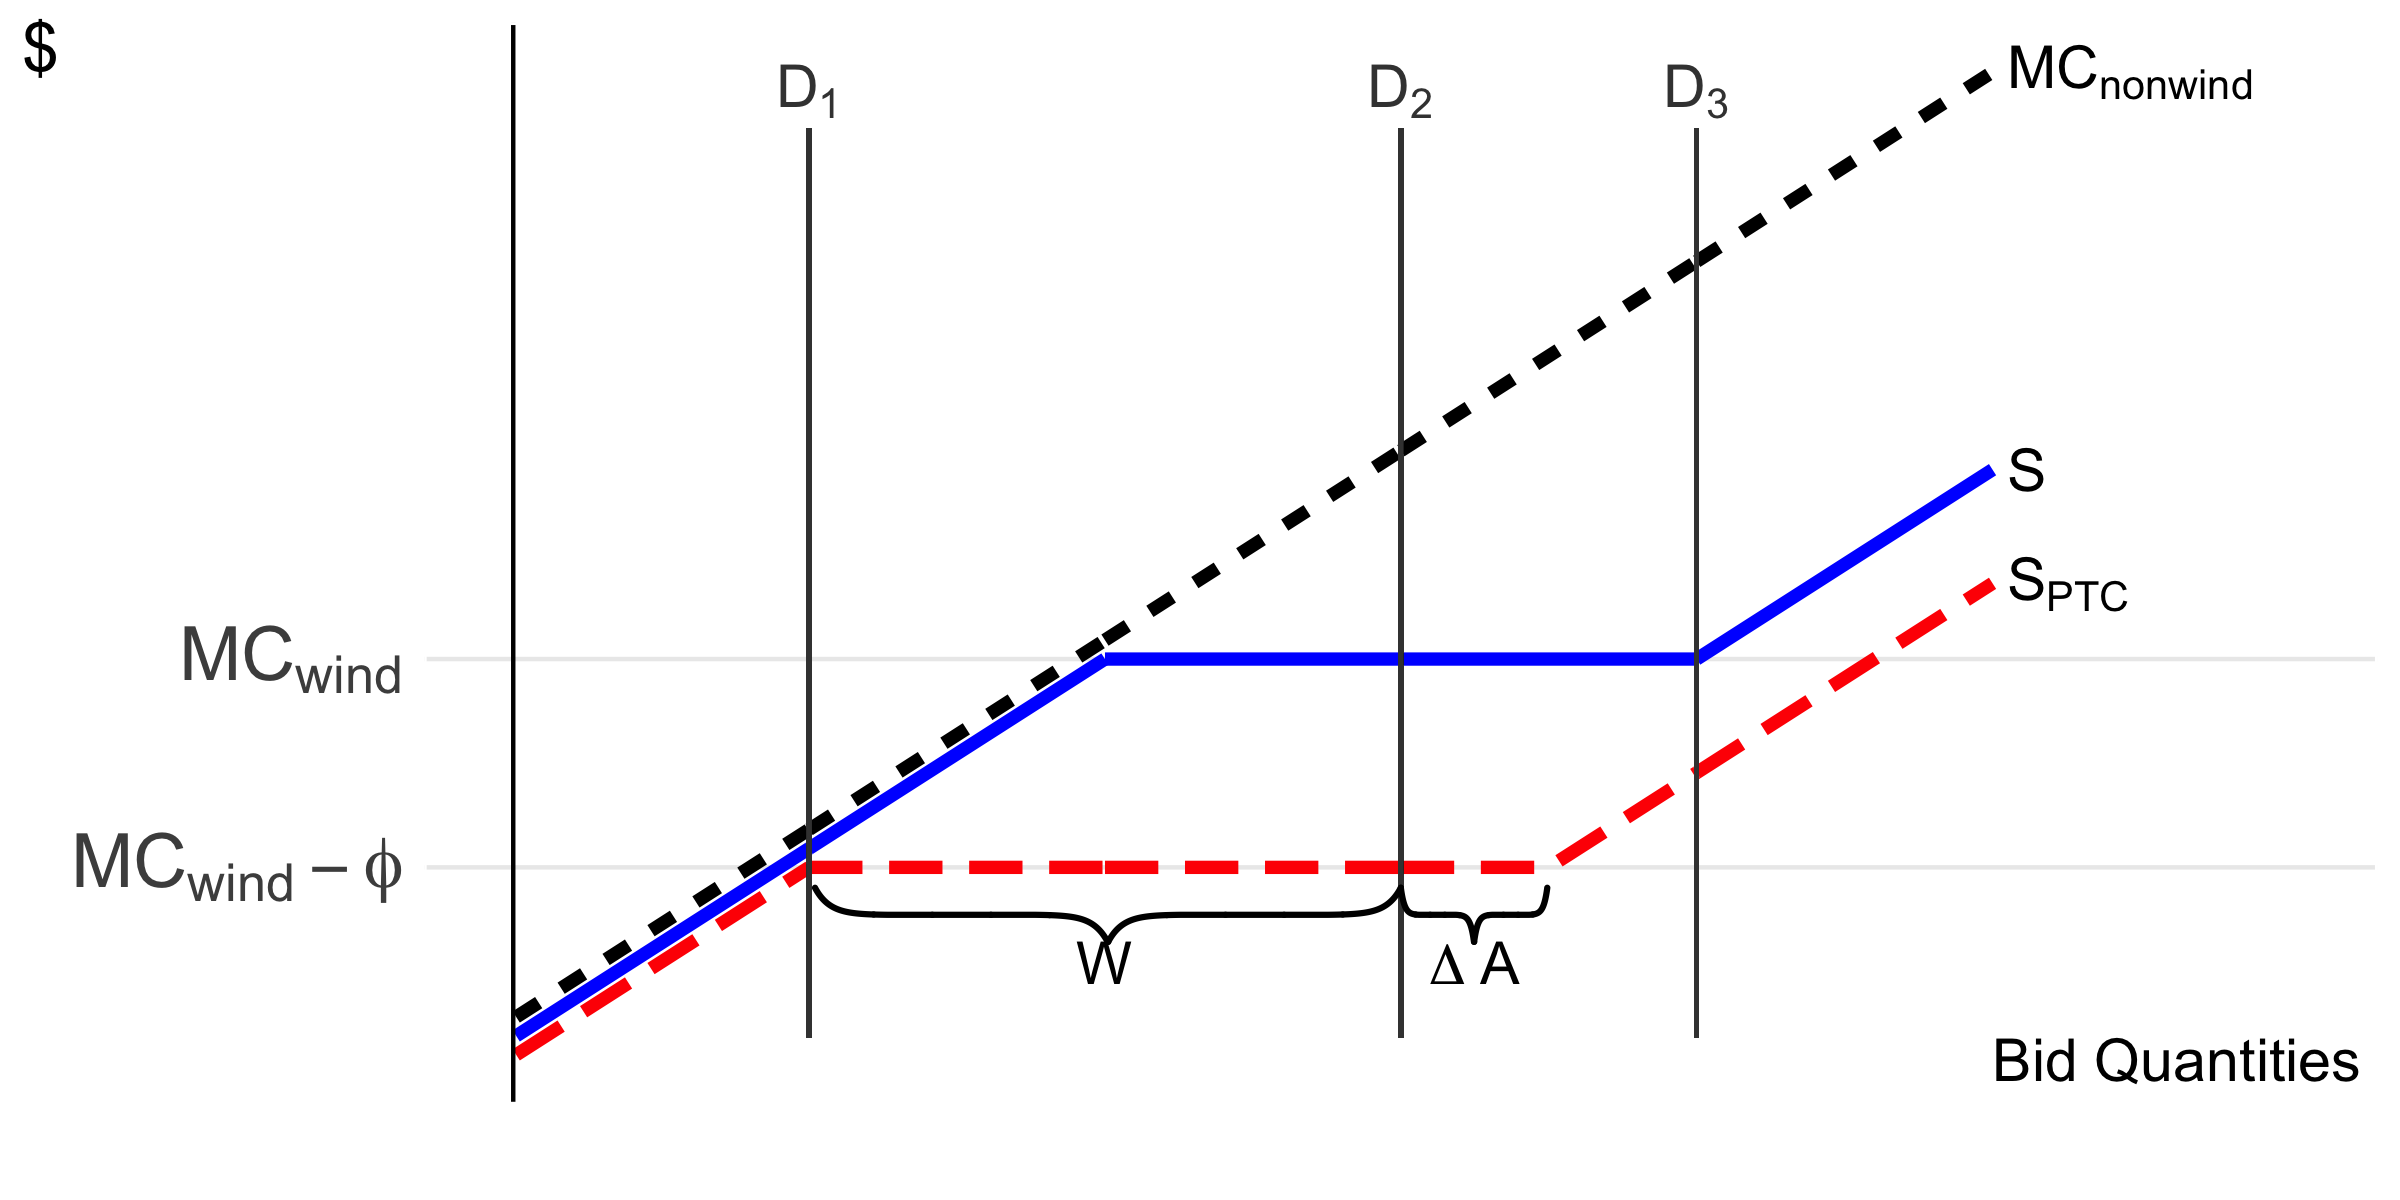
\includegraphics[width=0.85\textwidth]{dispatch.png}
\end{figure}

An output subsidy of $\phi$ per MWh of wind generation moves wind to the left in the dispatch curve, displacing some previously inframarginal non-wind capacity. This is because wind farms dispatched at a price of MC\textsubscript{wind}$-\phi$ will have net zero private marginal profits after accounting for the subsidy. The output subsidy also increases the availability of wind farms for the reasons discussed above. This boost in available capacity is represented by $\Delta A$. The resulting aggregate supply curve, which includes both wind and non-wind, is S\textsubscript{PTC}.

Comparing S and S\textsubscript{PTC} shows how, conditional on installed capacity, the net change in wind power generated, and the mechanism behind that change, depend on the level of demand. For very low levels of demand, below $D_1$, there is no difference in wind generation under the two subsidies because no wind is dispatched in either case. For demand between $D_1$ and $D_2$, the output subsidy increases wind generation via the dispatch effect. For demand between $D_2$ and $D_3$, the difference is due to both the dispatch and availability effects. Finally, for levels of demand above $D_3$, any difference in output across the two subsidy types comes entirely from the availability effect.

\section{Data\label{sec:Data}}

In this section, we concisely summarize our data sources and sample restrictions. Additional detail is provided in Appendix~\ref{sec:Data_Appendix}. We compiled data on wind farm characteristics and output from two publicly available Energy Information Administration (EIA) surveys covering all utility-scale wind farms in the United States. The EIA-860 database, which reflects an annual survey of power plants, contains: first date of commercial operation, operator, location, nameplate capacity, number of turbines, predominant turbine model, average annual wind speed,\footnote{We also refer to EIA's average annual wind speed as ``design wind speed'' to distinguish it from wind speed data from 3TIER.} wind quality class,\footnote{Wind quality class takes one of four categories defined by the International Electrotechnical Commission.} regulatory status of the plant,\footnote{EIA considers plants operated by entities that provide electricity within a designated franchised service area as regulated. Other plants are considered unregulated. There are exceptions to this rule but they do not apply to the plants analyzed in this study.} entity type of the principle owner,\footnote{The entity types recorded on Form EIA-860 are: cooperative, investor-owned utility, independent power producer, municipally-owned utility, political subdivision, federally-owned utility, state-owned utility, industrial, and commercial. We use this information to restrict our sample as described in the text. We also use it to construct a dummy variable for independent power producer (IPP) that we include in our analysis in order to capture variation in ownership structure conditional on regulatory status, as some non-regulated plants are owned by investor-owned utilities.} and operation within a regional transmission organization (RTO) or independent system operator (ISO). We combine this annual plant-level information with monthly electricity generation data collected through the Form EIA-923 survey of power plants.

We supplement these EIA data with proprietary data from the American Wind Energy Association (AWEA), 3TIER, and turbine manufacturers. The AWEA database contains additional cross-sectional information on each wind farm, including the wind turbine model and whether projects contract output through long-term power purchase agreements (PPAs) or sell on spot markets. We use the former to corroborate turbine data in the EIA-860 and the latter to construct ``offtake type'' indicator variables which control for potentially differential contracting arrangements across 1603 and PTC recipients in the estimated regression models.

3TIER uses global wind and weather monitor data to interpolate hourly wind speed, wind direction, air pressure, and temperature for the entire continental United States at a spatial resolution of approximately 5 kilometers.\footnote{For more information on how this dataset is constructed, see: \href{http://www.3tier.com/en/support/wind-prospecting-tools/how-was-data-behind-your-prospecting-map-created/}{http://www.3tier.com/en/support/wind-prospecting-tools/how-was-data-behind-your-prospecting-map-created/} (Accessed 2/14/2017).} We combine these high frequency wind data with power curves from turbine manufacturers for each turbine make and model in the EIA data.\footnote{Power curves were primarily obtained from \href{http://www.wind-power-program.com/}{http://www.wind-power-program.com/} (last accessed 2/14/2017), and supplemented with information obtained directly from turbine manufacturer marketing materials (generously provided to us by Joern Huenteler).} Using this information, we compute an ``engineering'' estimate of the potential output for each plant-month that accounts for the site-specific, nonlinear relationship between wind speeds and electricity generation. Further detail on this variable and its construction is provided in Appendix~\ref{Appendix:Potential-capacity-factor}.

The final dataset comes from the U.S. Department of Treasury. The dataset provides information on every large wind project recipient of a 1603 grant, including the amount awarded (equal to 30 percent of eligible investment costs), the date of the award, and the date placed in service.\footnote{The Department of the Treasury distinguished between ``large'' wind projects, which are eligible for the PTC, and ``small'' wind projects, which must have nameplate capacity no greater than 100 kilowatts and are eligible for investment tax credits. All utility-scale wind projects and all wind farms in the data compiled from the EIA fall into the ``large'' wind project category. } We assume that all developers of non-1603 recipient wind farms claimed the PTC based on both guidance provided by staff at the American Wind Energy Association and Internal Revenue Service data. Specifically, we confirmed that no corporation claimed the ITC for PTC-eligible projects (i.e., wind) over 2009-2012 in the annual Internal Revenue Service Estimated Data Line Counts reports for corporate tax returns. We do not have plant-specific tax data on the PTC claims, although we observe all power related data for presumed PTC-claimants through the EIA data described above.

Appendix table~\ref{tab:Summary-Statistics} presents an annual summary of these data for plants entering service between 2002 and 2014.\footnote{There are two potential ways to define online date based on the EIA data. One is the date that the survey respondent reports to EIA that the plant began commercial operation on Form EIA-860; the other is the first date that its generation appears in the EIA-923 production data. Although these by and large coincide, discrepancies can appear due to ``pre-commercial'' plant testing (923 date \textless{} 860 date) or due to the delay with which EIA begins tracking new plants (860 date \textless{} 923 date). This is important because the online date determines 1603 grant eligibility (our instrument). We use the 860 date, as we were told by an EIA expert that this date would be more accurate for our purposes. Nevertheless, IV results are robust to using the 923 date instead. In all specifications, plants with conflicting 923 and 860 dates around the 2009 eligibility cutoff are excluded from the sample.} In our empirical analysis, we restrict attention to plants with owners classified as either independent power producers or investor-owned utilities. Commercial and industrial facilities are excluded, as are plants that are publicly owned (e.g., municipal power plants), as these plants are not eligible for the PTC. We also exclude a small number of plants that appear to have claimed the PTC for some turbines that came online before 2009 and the Section 1603 grant for some turbines that came online in 2009 or later (see Appendix~\ref{sec:Data_Appendix} for further details).

Table~\ref{tab:ttest:ptcvs1603} compares projects placed into service during the 1603 grant eligibility period by subsidy type. Although the overall project sizes are comparable\textemdash both in terms of total size (i.e., nameplate capacity) and turbine size\textemdash 1603 recipients are located in areas with slightly lower average wind speeds, are less likely to be regulated, and are more likely to contract output through PPAs. Figure~\ref{map:2009to2012} presents a map of plant locations coded by subsidy choice. Although there is considerable spatial overlap in many parts of the U.S., some regions show a clear preference among developers for one subsidy type. Together, these differences are suggestive of selection.

Projects selecting the 1603 grant also have lower potential and realized capacity factors.\footnote{Capacity factors, which effectively measure power plant capacity utilization, are a commonly used metric of operational activity in the electric power sector \citep[see, for example,][]{davis_deregulation_2012}. Additional detail provided in Appendix~\ref{Appendix:Potential-capacity-factor}.} A capacity factor is the ratio of output to the maximum attainable output of a plant if it continuously produces electricity at its nameplate capacity. Here, the \textit{potential} capacity factor is an engineering-based prediction of the capacity factor computed using each plant's wind turbine and wind speed data. The \textit{realized} capacity factor (henceforth simply ``capacity factor'') is constructed using the plant's actual output. Thus, the final row of Table~\ref{tab:ttest:ptcvs1603} shows that 1603 recipients produce less electricity than PTC recipients on average, relative to their total potential output. In the next section, we describe our strategy for identifying the portion of this observed difference in productivity attributable to the subsidy rather than selection.

\begin{table}[h]
\caption{Comparison of 2009-2012 Projects by Policy Choice\label{tab:ttest:ptcvs1603}}
\begin{center}
\begin{tabular}{lcccc}
\hline \noalign{\smallskip} & PTC & 1603 & Difference & p-value\\
\noalign{\smallskip}\hline Nameplate Capacity (MW) & 102.27 & 92.03 & 10.24 & 0.30\\
Turbine Size (MW) & 1.84 & 1.91 & -0.07 & 0.20\\
Design Wind Speed (MPH) & 17.81 & 17.33 & 0.48 & 0.27\\
Regulated & 0.23 & 0.03 & 0.20 & 0.00\\
IPP & 0.68 & 0.89 & -0.21 & 0.00\\
PPA & 0.67 & 0.86 & -0.19 & 0.00\\
Potential Capacity Factor & 39.59 & 34.83 & 4.76 & 0.00\\
Capacity Factor & 36.76 & 30.61 & 6.15 & 0.00\\
\hline \noalign{\smallskip}New Wind Farms & 107 & 192 &  & \\
\noalign{\smallskip}\hline\end{tabular}\\
\end{center}

\footnotesize
Each row contains a two-sample t-test for a difference in means between recipients of the PTC and the Section 1603 grant that came online in 2009-2012 and are in the restricted sample described in Section~\ref{sec:Data}. Regulated, IPP, and PPA are binary variables. Potential Capacity Factor and Capacity Factor are ratios (scaled by 100), both of which are computed using data from 2013 and 2014.
\end{table}

\section{Empirical Strategy and Productivity Results \label{sec:Empirical-Strategy}}

Motivated by the previous discussion of the potential for output subsidies to increase wind farm productivity, we quantify the magnitude of this effect by estimating the following regression under several different assumptions and sample restrictions:

\begin{equation}
q_{it}=\delta D_{i}+\beta X_{it}+\nu_{it}\label{eq:second_stage}
\end{equation}
where $q_{it}$ is plant $i$'s capacity factor (in percentage points) in month-year $t$; $X_{it}$ is a vector of controls, such as engineering-based potential capacity factor, regulatory regime, presence of a power purchase agreement, and location dummies; and $D_i$ is an indicator for whether wind farm $i$ took the 1603 grant. The coefficient of interest, $\delta$, reflects the effect of \emph{removing} output subsidies. Given the preceding discussion of two channels through which output subsidies can increase production, we expect $\delta$ to be negative.

Estimating equation~\ref{eq:second_stage} using OLS is problematic due to the fact that wind farms had to opt in to the 1603 program, so $D_{i}$ was chosen. Intuitively, plants that expect to have high output relative to their investment costs will prefer the PTC, while plants with relatively high investment costs per unit of expected output will prefer the Section 1603 grant. Thus, OLS estimates could confound the response to reducing marginal production incentives with the fact that less productive plants are likely to have selected into the 1603 grant program. To address this concern, we employ two complementary empirical approaches to identify the causal effect of the Section 1603 grant on wind farm output: an instrumental variables estimator and a matching estimator.

\subsection{Instrumental Variable Estimation}

Our primary empirical strategy harnesses the natural experiment created by the 1603 grant program by comparing wind farms that came online just before and just after the program went into effect. While the Section 1603 grant was not randomly assigned, its creation came as a plausibly exogenous shock to the industry. We exploit this shock by using a binary indicator for whether the project came online after January 1, 2009 as an instrument for cash grant recipient status. We use this instrument along with wind farms' monthly output data over 2010-2014 to estimate equation~\ref{eq:second_stage} via two-stage least squares. This IV approach is similar to a fuzzy regression discontinuity design with time as the running variable, which we implement as a sensitivity analysis in Appendix Table~\ref{tab:rdd_cf_linear}.

Identification and interpretation of $\delta$ relies on two key assumptions: (1) that ineligible firms cannot manipulate the date they came online to receive the subsidy, and (2) that the instrument (subsidy eligibility) only affects outcomes through its effect on the endogenous variable (subsidy choice).\footnote{Identification and interpretation as a local average treatment effect also relies on three other restrictions/assumptions. First, we know from the data that the first stage is non-zero. Second, the monotonicity assumption holds by virtue of the policy environment: firms cannot ``defy'' treatment assignment because the 1603 grant is only available from the Federal government. Finally, we assume homogeneous treatment effects.} The first assumption is supported by institutional details. Wind farms could not strategically adjust when they came online in anticipation of the policy, as the policy had not even been proposed until after the January 1, 2009 eligibility date (see Section~\ref{subsec:RenewablePolicies}). 

To assuage concerns about the exclusion restriction, our main IV specification uses a bandwidth of one year on either side of the start date of the policy, relying only on a comparison of projects that came online in 2008 and 2009. This has two main advantages. First, long-run trends in wind turbine technology and electricity markets are less likely to influence our results. For example, $82$ percent of the new projects in our 2008-2009 sample use turbine models that were used in both years. Second, projects that came online in early 2009 were planned and began construction in 2008 (or earlier), which implies that these plants were originally designed for the PTC \citep{bolinger_preliminary_2010}. This helps mitigate concern that 1603 grant recipients are fundamentally different, as may be the case in later periods. 

Table~\ref{tab:ttest_RD_sample_pre} compares projects coming online in 2008 with those coming online in 2009 using two-sample t-tests. In contrast to the comparison of PTC and 1603 plants over the full life of the policy (Table~\ref{tab:ttest:ptcvs1603}), the two groups in Table~\ref{tab:ttest_RD_sample_pre} are statistically indistinguishable in terms of several pre-treatment characteristics including turbine size, wind speed, regulatory status, and whether a wind farm has entered into a PPA. Similarly, despite small differences in subsidy preference across regions in 2009, Figure~\ref{map:2008to2009} shows that both subsidy types have strong spatial overlap with PTC plants that came online in 2008, which is the relevant comparison in this analysis. Nonetheless, capacity and the probability of being an independent power producer are statistically different in Table~\ref{tab:ttest_RD_sample_pre} across these two years. To account for this, we condition on these variables in our regressions. 

\begin{table}[H]
\caption{Projects Entering One Year Before and After the Policy\label{tab:ttest_RD_sample_pre}}
\begin{center}
\begin{tabular}{lcccc}
\hline \noalign{\smallskip} & 2008 & 2009 & Difference & p-value\\
\noalign{\smallskip}\hline Nameplate Capacity (MW) & 85.97 & 110.73 & -24.77 & 0.05\\
Turbine Size (MW) & 1.82 & 1.81 & 0.00 & 0.95\\
Design Wind Speed (MPH) & 18.01 & 17.50 & 0.52 & 0.29\\
Regulated & 0.13 & 0.12 & 0.01 & 0.81\\
IPP & 0.58 & 0.79 & -0.21 & 0.01\\
PPA & 0.75 & 0.74 & 0.01 & 0.85\\
Potential Capacity Factor & 37.50 & 37.24 & 0.27 & 0.84\\
Capacity Factor & 34.47 & 31.85 & 2.62 & 0.01\\
\hline \noalign{\smallskip}New Wind Farms & 69 & 77 &  & \\
1603 Recipients  & 0 & 51 &  & \\
\noalign{\smallskip}\hline\end{tabular}\\
\end{center}

\footnotesize
Each row contains a two-sample t-test for a difference in means between wind farms that came online in 2008 and in 2009 and that are in the restricted sample described in Section~\ref{sec:Data}. Regulated, IPP, and PPA are binary variables. Potential Capacity Factor and Capacity Factor are ratios (scaled by 100), both of which are computed using data from 2013 and 2014.
\end{table}

Most importantly, the plants in these two years have remarkably similar engineering-based potential capacity factors. However, our outcome variable, \textit{realized} capacity factor, is lower (and statistically distinguishable) for projects coming online in 2009 than for projects coming online in 2008. This difference in observed productivity, despite the lack of difference in potential productivity, provides an (unscaled) preview of the main IV results. 

\subsubsection*{Results \label{sec:results:rd}}

Table~\ref{tab:rdd_cf} reports the instrumental variable results. The sample is restricted to a balanced panel of monthly generation from 2010 to 2014 at wind farms that came online in 2008 or 2009. The dependent variable in each regression is the capacity factor in percentage points.

\begin{table}[h]
\caption{Instrumental Variables Estimates \label{tab:rdd_cf}}
\begin{center} {\footnotesize{}{
\def\sym#1{\ifmmode^{#1}\else\(^{#1}\)\fi}
\begin{tabular}{l*{6}{c}}
\toprule
                &\multicolumn{1}{c}{(1)}         &\multicolumn{1}{c}{(2)}         &\multicolumn{1}{c}{(3)}         &\multicolumn{1}{c}{(4)}         &\multicolumn{1}{c}{(5)}         &\multicolumn{1}{c}{(6)}         \\
\midrule
1603 Grant      &   -5.148\sym{***}&   -3.626\sym{***}&   -2.842\sym{***}&   -3.697\sym{***}&   -2.893\sym{**} &   -3.156\sym{***}\\
                &  (0.915)         &  (0.899)         &  (0.829)         &  (1.351)         &  (1.238)         &  (1.170)         \\
\addlinespace
Regulated       &                  &   -1.562         &   -5.439\sym{***}&                  &   -1.371         &   -5.446\sym{***}\\
                &                  &  (1.712)         &  (1.979)         &                  &  (1.685)         &  (1.970)         \\
\addlinespace
PPA             &                  &   -0.648         &   -2.608\sym{***}&                  &   -0.600         &   -2.618\sym{***}\\
                &                  &  (1.048)         &  (0.927)         &                  &  (1.056)         &  (0.925)         \\
\addlinespace
IPP             &                  &   -1.350         &   -2.554\sym{*}  &                  &   -1.408         &   -2.514\sym{*}  \\
                &                  &  (1.333)         &  (1.351)         &                  &  (1.305)         &  (1.307)         \\
\addlinespace
Potential Capacity Factor&                  &    0.501\sym{***}&    0.551\sym{***}&                  &    0.503\sym{***}&    0.553\sym{***}\\
                &                  & (0.0366)         & (0.0391)         &                  & (0.0368)         & (0.0386)         \\
\addlinespace
Var(Wind Speed) &                  &   0.0400         &   -0.426\sym{***}&                  &   0.0637         &   -0.432\sym{***}\\
                &                  &  (0.148)         &  (0.103)         &                  &  (0.155)         &  (0.107)         \\
\addlinespace
log(Capacity)   &                  &   -0.567         &    0.571         &                  &   -0.605         &    0.580         \\
                &                  &  (0.429)         &  (0.471)         &                  &  (0.430)         &  (0.470)         \\
\midrule
Regression Type &      OLS         &      OLS         &      OLS         &     2SLS         &     2SLS         &     2SLS         \\
Controls        &        N         &        Y         &        Y         &        N         &        Y         &        Y         \\
State FE        &        N         &        N         &        Y         &        N         &        N         &        Y         \\
R-sq.           &    0.372         &    0.557         &    0.660         &        -         &        -         &        -         \\
N               &     8752         &     8752         &     8752         &     8752         &     8752         &     8752         \\
First-stage F-stat.&                  &                  &                  &      148         &      169         &      113         \\
\bottomrule
\end{tabular}
}
} \end{center}
\footnotesize
The dependent variable is the capacity factor in percentage points. Data include a balanced panel of monthly observations from 2010 to 2014 for all wind farms. All models contain year-month dummies. Standard errors, clustered at the plant level, are reported in parentheses.
\end{table}

The primary coefficient of interest ($\delta$) appears in the first row of the table, labeled 1603 Grant. The first three columns present OLS estimates of equation~\ref{eq:second_stage}. Column 1 includes only time (month-year) dummies. The interpretation is that plants receiving output subsidies operated at 5 percentage points lower capacity factor compared to PTC recipients coming online between 2008 and 2009. Column 2 adds controls for plant size and monthly wind quality, as well as dummies for whether the plant is regulated, whether it is owned by an independent power producer, and presence of a power purchase agreement.\footnote{Unless otherwise noted, the same controls appear in every model throughout the paper. Additional discussion of the potential capacity factor and wind speed variables is provided in Appendix~\ref{Appendix:Potential-capacity-factor}.} Consistent with the descriptive evidence above, 1603 and PTC plants differ on observable dimensions, and controlling for these differences reduces the estimated productivity gap. Column 3 adds state fixed effects to account for other unobserved differences in markets and renewable policies across states, which attenuates the relationship further.

Columns 4-6 present IV estimates using the same covariates, instrumenting for 1603 receipt with an indicator for whether the wind farm was eligible for the 1603 program. Conditioning only on month of sample, 1603 plants are 3.7 percentage points less productive than their PTC counterparts. This difference is considerably smaller than the OLS estimate in column 1. Adding controls results in a modestly lower estimated 1603 effect of 2.9 percentage points, and is our preferred specification. Column 6 adds state fixed effects, which effectively discards 25 percent of the sample for which there is no within-state subsidy variation. The estimate splits the difference between the previous two, leaving a 3.2 percentage point gap in productivity across plants choosing the two subsidy types. Our preferred estimate of 2.89implies that 1603 grant recipients would have produced roughly 10percent more power had they claimed the PTC.\footnote{This 10 percent reduction is computed by dividing the estimated 2.89percentage point reduction in capacity factor by the average capacity factor for all 1603 grant recipients of 30.32percentage points.} To provide context for the magnitude of this estimate, note that it is in line with industry claims for how post-construction wind farm optimization services could increase output (see discussion in Section~\ref{sec: Background}). The marginal incentive of the PTC is quite substantial during this time period, providing a premium of roughly 40 percent over the average price of power sold by wind farms to the grid. As such, the estimate in column 5 implies a supply elasticity of around 0.25. 

\subsubsection*{Robustness Analysis}

We assess the sensitivity of our results to the assumed sample bandwidth. The primary motivation for doing this is concern about violations of the exclusion restriction. Since our instrument is based on time, we implicitly assume that the time a plant was placed into operation only affects productivity through the change in subsidy margin. This assumption could fail if there were changes between 2008 and 2009 in the way plants were initially set up that had persistent effects on productivity. Although we believe it is highly unlikely that wind farm developers could have made significant changes to projects that began operations in 2009 after first learning about the policy, that possibility becomes more remote as we shorten the sample around the policy introduction. Of course, smaller bandwidths generate smaller samples, lessening the statistical precision of our estimates. 

Figure~\ref{fig:CFbandwidths} presents coefficients from the preferred specification in column 5 in graphical form using alternative bandwidths ranging from three months to 24 months on each side of the policy change. Although the confidence intervals are large for the very small bandwidths, the results are consistent and reinforce our baseline findings: all specifications suggest receipt of the 1603 grant leads firms to produce less electricity than they would have if they had received the PTC. Moreover, the fact that the point estimates remain remarkably stable between nine and 24 months assuages concerns that the results are driven by time trends.\footnote{We also estimate models that allow for the possibility of trends within the 2008-2009 time period in technology, site quality, and other factors that have persistent effects on output. Table~\ref{tab:rdd_cf_linear} presents results from a parametric fuzzy regression discontinuity model that includes piecewise linear trends. Unfortunately, given the small sample size, these results are quite noisy. In models 4 and 5, the point estimates are larger in magnitude than the IV estimates, while in model 6 the results are smaller and not statistically distinguishable from either the IV estimates or zero. The variability in these estimates may be the result of weak instruments, as they have relatively small first-stage F-statistics.}

\begin{figure}[H]
\caption{IV Estimates using Alternative Bandwidths \label{fig:CFbandwidths}}
\vspace{-15pt}
\begin{center}
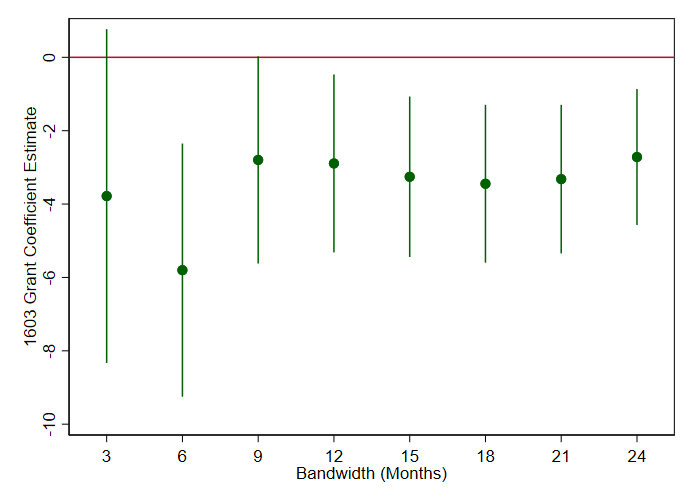
\includegraphics[width=0.7\textwidth]{fuzzyRDD_capfactor_bandwidths_nostateFEs.png}
\end{center}
\vspace{-15pt}
\footnotesize
Coefficient estimates from 2SLS regressions of capacity factor on a binary indicator for 1603 grant receipt, instrumented with a binary indicator for grant eligibility. Regressions also include year-month dummies, controls for plant size and wind quality, as well as dummies for whether the plant is regulated, is owned by an IPP, and has a PPA. Data are a panel of monthly observations from 2010 to 2014. Each point corresponds to a sample defined by its bandwidth around January 1, 2009, so that the leftmost model includes plants that came online between October 2008 and March 2009, and the rightmost model includes plants that came online between January 2007 and December 2010. A bandwidth of 12 months corresponds to column 5 of Table \ref{tab:rdd_cf}. Spikes denote 95\% confidence intervals based on standard errors clustered at the plant level.
\end{figure}


\subsection{Matched Differencing \label{subsec:Matching}}

Our second empirical strategy uses a combination of matching and differencing to infer counterfactual outcomes for 1603 grant recipients. Assume the unobserved component of production takes the form $\nu_{it}=A_{i}+\epsilon_{it}$, where $A_{i}$ denotes the unobserved quality of wind farm $i$. Selection in our context would manifest itself as a correlation between $A_{i}$ and $D_{i}$. Conditioning on $A_{i}$ would eliminate this bias, as $E[q_{it}|X_{it},A_{i},D_{i}=1]$=$E[q_{it}|X_{it},A_{i},D_{i}=0]+\delta$. Under the assumption that $A_{i}$ is time-invariant, the use of plant fixed effects with panel data would remove this bias.

Since subsidies are irreversibly chosen at the commencement of operations, we do not observe subsidy variation within a plant, and thus cannot include plant fixed effects. Instead, we adopt the additional assumption that unobserved heterogeneity takes the following form, $A_{i}=g(X_{i})+\gamma Post_{i}$, where $g()$ is an unknown function of observable wind farm characteristics, and $\gamma$ is a wind farm vintage fixed effect for plants entering post-ARRA. Although $g()$ is unknown, including a dummy variable for each unique combination of characteristics $X_{i}$ would fit any $g()$. The difference in productivity between two wind farms with the same characteristics that entered in different policy periods would then simply be $\gamma$.

While we cannot fit $g()$ exactly given that $X_{i}$ contains continuous covariates and our sample is finite, we approximate $g()$ by matching wind farms with similar characteristics across different vintages. We divide our sample into two groups corresponding to two policy regimes: wind farms that entered between 2005 and 2008 (``pre'' plants), when there was no subsidy choice, and wind farms that entered between 2009 and 2012 (``post'' plants), which could choose either the PTC or the 1603 grant. We then match pre and post wind farms on observable characteristics using coarsened exact matching.\footnote{\citet{iacus_causal_2012} outline the algorithm and derive its statistical properties. More information and implementation packages can be found at \href{http://gking.harvard.edu/cem}{http://gking.harvard.edu/cem}.} Let $g$ index a group of pre and post plants that are matched together. Equation~\ref{eq:second_stage} becomes, 

\begin{equation}
q_{it}=\delta D_{i}+\beta X_{it}+A_{g}+\gamma Post_{i}+\epsilon_{it}\label{eq:mdd} ,
\end{equation}
where $Post_{i}$ is an indicator for whether a plant came online after the 1603 program was introduced. Intuitively, the estimator takes the average difference between 1603 recipients and their pre-period matched counterparts, and subtracts the difference between post-period PTC plants and matched pre-plants within their group. To see this, let $D_{g}$ indicate the \emph{observed} subsidy choice of the post-period plants in group $g$. Then
\[
E[q_{it}|D_{g}=0,Post_{i}=1]-E[q_{it}|D_{g}=0,Post_{i}=0]=\gamma
\]
\[
E[q_{it}|D_{g}=1,Post_{i}=1]-E[q_{it}|D_{g}=1,Post_{i}=0]=\gamma+\delta
\]
In practice, we replace $\gamma$ with fixed effects for cohort (i.e., the first year each wind farm generated electricity), and allow group-level unobservables to vary by time.

Matching requires us to drop plants that do not lie within the common support of pre and post period entrants on key observable dimensions. Within the set of plants that remain, identification requires assuming there are no unobservables that affect both production changes across pre and post plants and subsidy choice (i.e., unconfoundedness). We also assume the covariates used for matching are unaffected by the availability of the 1603 grant. While we cannot directly assess this assumption, the long development timeline of wind farms reduces concern over any large responses on this dimension. Moreover, the IV analysis addresses precisely this concern.

The primary concern with the IV estimator is that the instrument, time, may be picking up other trending factors that affect productivity. Our matching estimator relaxes this by allowing unobservable dimensions of wind farm entry cohorts to evolve over time. The key assumption is parallel trends in these unobservable factors across the types of plants that choose each subsidy in the post period. 

\subsubsection*{Results \label{sec:results:matching}}

We match exactly on several categorical variables (geography, wind quality class, regulatory status, and entity type) and two coarsened continuous variables (capacity and design wind speed).\footnote{In this analysis, we match on two wind quality measures collected by the EIA, design wind speed and wind class. An alternative would be to match on the realized potential capacity factor, which we construct and use as a control at the month level, averaged over the sample. We prefer the EIA measures because they are directly reported to the EIA, and likely more accurate in the cross section. These two measures are also widely used in the industry, with wind class (a categorization of site wind variability) used as a critical determinant of which turbines can safely be placed at a location. Moreover, the conceptual exercise here is to match similar \textit{sites} in the pre and post policy period, whereas the potential capacity factor confounds site-specific characteristics with project-specific characteristics like turbine technology that may vary over time and could be influenced by the policy itself. With that said, the results are qualitatively similar when we match on potential capacity factor instead. These are presented in appendix Table~\ref{tab:matching_group_ptnlcf}.} This procedure selects all pre-period wind farms within the same coarsened cell in the covariate space as each post-period wind farm.

Table~\ref{tab:matching_balance} compares pre- and post-period entrants after using coarsened exact matching with state as the geography. Of the 465 wind farms in our sample entering between 2005 and 2012, 204 lie within the common support of these variables across the two policy periods.\footnote{The number of post-period matches is higher than pre-period matches because more post-period plants fall within the same coarsened cell than do pre-period plants.} The number of post-period 1603 matches is about double the number of PTC matches, which is in line with their underlying population probabilities. T-tests confirm that this restricted sample is in fact balanced across the two time periods on the matched dimensions. In particular, the two dimensions that were imbalanced in the IV sample, capacity and IPP status, are now statistically equivalent across the pre and post periods in this sample by construction. 

\begin{table}[h]
\caption{Matching Balance \label{tab:matching_balance}}
\begin{center}
\begin{tabular}{lcccc}
\hline \noalign{\smallskip} & Pre & Post & Difference & p-value\\
\noalign{\smallskip}\hline Nameplate Capacity (MW) & 101.91 & 105.39 & 3.48 & 0.74\\
Turbine Size (MW) & 1.78 & 1.89 & 0.11 & 0.05\\
Design Wind Speed (MPH) & 17.92 & 17.46 & -0.45 & 0.14\\
Regulated & 0.09 & 0.09 & 0.00 & 1.00\\
IPP & 0.89 & 0.89 & 0.00 & 1.00\\
PPA & 0.82 & 0.77 & -0.05 & 0.42\\
Potential Capacity Factor & 36.76 & 37.39 & 0.63 & 0.53\\
Capacity Factor & 34.01 & 32.80 & -1.21 & 0.14\\
\hline \noalign{\smallskip}Wind Farms & 86 & 118 &  & \\
1603 Recipients &  & 83 &  & \\
\noalign{\smallskip}\hline\end{tabular}\\
\end{center}

\footnotesize
Each row contains a two-sample t-test for a difference in means between wind farms that came online before versus after January 1, 2009 that meet sample restrictions described in Section~\ref{sec:Data} and are selected using coarsened exact matching. See text for more details on the matching procedure. Regulated and IPP are identical across samples by construction. Regulated, IPP, and PPA are binary variables. Potential Capacity Factor and Capacity Factor are ratios (scaled by 100), both of which are computed using data from 2013 and 2014.
\end{table}

Table~\ref{tab:matching_group} reports the results from regressions estimated through variations of this matching strategy with an unbalanced panel of monthly wind farm production data from 2009 to 2014. As before, the dependent variable in each regression is the capacity factor measured in percentage points. All models include the same controls as our preferred IV regressions as well as dummies for cohort (i.e., the first year each wind farm generated electricity). Column 1 presents estimates from estimating OLS on the full sample including all 465 wind farms entering during the pre- or post-period. Column 2 restricts the sample to plants matched across periods. Column 3 includes matched group fixed effects. Column 4 interacts those group fixed effects with year of sample, allowing for unobserved factors that affect specific groups and vary over time. Column 5 includes group-year-month fixed effects. 

Simply restricting the sample to observably similar plants across periods increases the estimated impact of the 1603 grant from 2.9 to 4 percentage points. This suggests that there are low productivity PTC plants and/or high productivity 1603 plants that do not lie in the common support across periods. Allowing for increasingly time-varying group level unobservables has remarkably little effect on the estimates. The estimated productivity reduction in column 4 of 3.72percentage points (12percent) is similar to our preferred IV estimate, despite relying on different identifying assumptions.

\begin{table}[h]
\begin{center}
\caption{Matching Estimates \label{tab:matching_group}}
{
\def\sym#1{\ifmmode^{#1}\else\(^{#1}\)\fi}
\begin{tabular}{l*{5}{c}}
\toprule
                    &\multicolumn{1}{c}{(1)}         &\multicolumn{1}{c}{(2)}         &\multicolumn{1}{c}{(3)}         &\multicolumn{1}{c}{(4)}         &\multicolumn{1}{c}{(5)}         \\
\midrule
1603 Grant          &      -2.942\sym{***}&      -3.975\sym{***}&      -3.862\sym{***}&      -3.716\sym{***}&      -3.633\sym{***}\\
                    &     (0.719)         &     (1.063)         &     (1.019)         &     (1.033)         &     (1.159)         \\
\midrule
Sample              &         All         &     Matched         &     Matched         &     Matched         &     Matched         \\
FEs                 &       State         &       State         &       Group         &     Group*Y         &   Group*Y*M         \\
R-sq.               &       0.615         &       0.623         &       0.632         &       0.642         &       0.762         \\
N                   &       21303         &       10106         &       10106         &       10106         &       10106         \\
\bottomrule
\end{tabular}
}

\end{center}
\footnotesize
The matched sample was constructed using coarsened exact matching on state, wind quality class, regulatory status, entity type, capacity, and design wind speed. All models include the controls listed in the IV models in Table~\ref{tab:rdd_cf}: log capacity, potential capacity factor, and wind speed variance, as well as dummies for whether the plant is regulated, whether it is an IPP, the presence of a PPA, and month of sample. All models also include cohort dummies. Models are estimated using an unbalanced panel of monthly wind farm production data from 2009 to 2014. Standard errors, clustered at the plant level, are reported in parentheses.
\end{table}

\subsubsection*{Robustness Analysis}

The most restrictive matching criteria in the previous exercise is the requirement that pre and post plants be in the same state. In order to explore the impact of this assumption, and to incorporate more plants into the analysis, we re-estimate the model from column 4 under different geographic restrictions (Table~\ref{tab:matching_table_cf}). As above, all models use coarsened exact matching on geography, wind quality class, regulatory status, entity type, capacity, and design wind speed. In addition, column 1 matches on NERC region as well as an indicator for whether the plant is in an ISO. Column 2 matches on the specific ISO a plant participates in, and column 3 matches on both NERC region and ISO. Finally, column 4 matches on state, repeating column 4 from the previous table. In addition to controls, month of sample dummies, and matched group-year dummies, each of the first three models also include state fixed effects to account for differences in state-level renewable policies. As in the previous table, the results increase slightly as increasing restrictions are placed on the matching procedure. However, we cannot statistically distinguish among the coefficient estimates.

\begin{table}[H]
\begin{center}
\caption{Sensitivity of Matching Estimates to Geographic Restrictions \label{tab:matching_table_cf}}
{
\def\sym#1{\ifmmode^{#1}\else\(^{#1}\)\fi}
\begin{tabular}{l*{4}{c}}
\toprule
                    &\multicolumn{1}{c}{(1)}         &\multicolumn{1}{c}{(2)}         &\multicolumn{1}{c}{(3)}         &\multicolumn{1}{c}{(4)}         \\
\midrule
1603 Grant          &      -2.989\sym{***}&      -3.362\sym{***}&      -3.472\sym{***}&      -3.716\sym{***}\\
                    &     (0.918)         &     (0.961)         &     (1.032)         &     (1.033)         \\
\midrule
\# Pre-PTC          &         108         &         100         &          90         &          86         \\
\# Post-PTC         &          54         &          51         &          44         &          35         \\
\# Post-1603        &         116         &          87         &          78         &          83         \\
Region              & Nerc-1(ISO)         &         ISO         &    Nerc*ISO         &       State         \\
R-sq.               &       0.634         &       0.677         &       0.661         &       0.642         \\
N                   &       13439         &       11724         &       10577         &       10106         \\
\bottomrule
\end{tabular}
}

\end{center}
\footnotesize
Matched samples constructed using coarsened exact matching on geographies listed in the table, wind quality class, regulatory status, entity type, capacity, and design wind speed. All models include the controls listed in the IV models in Table~\ref{tab:rdd_cf}: log capacity, potential capacity factor, and wind speed variance, as well as dummies for whether the plant is regulated, whether it is an IPP, the presence of a PPA, and month of sample. All models also include cohort dummies, matched group-year fixed effects, and state fixed effects. Models are estimated using an unbalanced panel of monthly wind farm production data from 2009 to 2014. Standard errors, clustered at the plant level, are reported in parentheses.
\end{table}

\section{Discussion \label{sec:Discussion}}


\subsection{Mechanism and Interpretation \label{sec:Mechanism}}

We estimate that selecting the 1603 grant, an investment subsidy, caused wind farms to produce about 10percent less output than they would have under the PTC, an output subsidy. As discussed in Section \ref{subsec:outputModel}, this result could reflect a ``dispatch'' effect -- wind displacing some previously inframarginal generation at low demand levels -- and an ``availability'' effect -- wind displacing marginal generation at all other demand levels.

How much of the estimated difference in output across PTC and 1603 plants can be attributed to each mechanism? Data limitations hinder direct evaluations of these mechanisms. Many companies tout wind farm services which promise productivity increases that are similar in magnitude to our estimated treatment effect.\footnote{For example, General Electric offers a product called ``PowerUp'', which it describes as ``a customized suite of software and hardware-enabled technologies created to increase a wind farm's output by up to 10\%, taking into account environmental conditions.'' Source: \href{https://www.gerenewableenergy.com/wind-energy/turbine-services/platform-upgrades}{General Electric website} (accessed 1/29/2018).} We cannot formally test for the impact of 1603 grant receipt on the adoption of these services, as a measure of the availability effect, because we do not observe such expenditures. Similarly, we cannot directly estimate separate treatment effects during periods of low and high demand when the dispatch effect would be more and less important, since we only observe plant output on a monthly basis.

However, by using hourly electricity prices and our engineering-based \emph{potential} output measure, we can approximate the share of our estimated productivity effect plausibly caused by the dispatch effect. We focus on periods when wind plants face negative electricity prices. Absent the PTC or other output incentives, a wind farm should bid into a power market at a price of zero. Thus, negative prices are a useful proxy for periods during which demand is sufficiently low that the dispatch effect could dominate any output differences between PTC and 1603 plants (see Figure \ref{fig:dispatch}).

First, we compute the share of hours with prices below zero and the amount of potential output during those hours, by plant and month. For six of the seven ISOs represented in our sample, we match hourly location-specific (nodal) electricity prices to our wind plants.\footnote{Nodal price information was not available from SPP. Data prior to 2011 was not available for all ISOs.} On average across PTC plants over 2011-2014, we find that negative prices occur about 5.8 \unskip percent of the time, and correspond to a potential capacity factor of 3.5 \unskip over a month. In contrast, 1603 plants face negative prices about 3.6 \unskip percent of the time, and these periods have a potential capacity factor of about 2.0 \unskip over a month. With our monthly average capacity factor treatment effect of 2.89 \unskip (IV) to 3.72 \unskip (matching), the potential capacity factor during negative price hours at 1603 plants is large enough to explain up to two-thirds of our estimated output effect.

Plants claiming 1603 grants, however, may operate when electricity prices fall below zero for several reasons: state renewable portfolio standards indirectly subsidize output, and ``green'' long-term contracts can encourage operation even when prices in the wholesale market are negative. To quantify the potential impact of these incentives, we estimate the following regression, 
\begin{align*} \label{eq:ptnl_cf_regs}
  q_{it}= &1\{D_i = 0 \} \left( \alpha_{PTC} \mbox{Potential CF}_{it} + \beta_{PTC} \mbox{Negative Price Potential CF}_{it} \right) + \\
      &1\{D_i = 1 \} \left( \alpha_{1603} \mbox{Potential CF}_{it} + \beta_{1603} \mbox{Negative Price Potential CF}_{it} \right) + \mu_{i} + \eta_{t} +\epsilon_{it} , 
\end{align*}
where $q_{it}$ is the observed capacity factor for plant $i$ in month $t$, and $D_i$ is an indicator for whether plant $i$ took the 1603 grant. Potential CF is the engineering-based potential capacity factor computed using data for all hours in each month. Negative Price Potential CF is computed in a similar way, except that the numerator only includes potential output during hours in which the price at the closest node is less than zero, while the denominator is still computed using all the hours in a month. As a result, the coefficient on Negative Price Potential CF can be interpreted as the differential effect of potential output on realized output during negative price hours. The model includes plant ($\mu_i$) and month of sample ($\eta_t$) fixed effects. 

Table \ref{tab:PlantNegativeCFRegs} presents the results. For PTC plants, a one percentage point increase in potential capacity factor is associated with a $0.74$ percentage point increase in observed capacity factor (within plant). The small and statistically insignificant coefficient on Negative Price Potential CF for PTC plants indicates that the relationship between potential and observed capacity factors does not change during negative price hours. The 1603 plants' potential capacity factors are associated with smaller levels of observed capacity factor than for the PTC plants ($0.68$ vs. $0.74$), consistent with these plants being less productive. However, unlike at PTC plants, this association is roughly half as large for negative price hours ($\hat{\alpha}_{1603} + \hat{\beta}_{1603} = 0.68-0.32 = 0.36$). The significant difference in Negative Price Potential CF coefficients suggests PTC plants behave differently than 1603 plants during negative price hours, consistent with the dispatch effect. The sum of the two coefficient estimates for 1603 plants, however, is economically significant, suggesting that 1603 plants do produce power frequently -- perhaps more than half of the time -- when prices are negative.

\begin{table}[H]
  \caption{Potential Output and Observed Output by Plant Type \label{tab:PlantNegativeCFRegs}}
  \begin{center}
    \footnotesize{
    {
\def\sym#1{\ifmmode^{#1}\else\(^{#1}\)\fi}
\begin{tabular}{l*{1}{c}}
\toprule
                &\multicolumn{1}{c}{Observed Capacity Factor}\\
\midrule
PTC - Potential Capacity Factor&    0.740\sym{***}\\
                & (0.0335)         \\
\addlinespace
PTC - Negative Price Potential Capacity Factor&   0.0416         \\
                & (0.0405)         \\
\addlinespace
1603 - Potential Capacity Factor&    0.682\sym{***}\\
                & (0.0327)         \\
\addlinespace
1603 - Negative Price Potential Capacity Factor&   -0.325\sym{***}\\
                & (0.0909)         \\
\midrule
Observations    &    12468         \\
\bottomrule
\end{tabular}
}

    }
  \end{center}
  \footnotesize
  Plant sample contains 120 \unskip 1603 plants and 177 \unskip PTC plants that entered between 2005 and 2012, in ISOs for which we obtained locational marginal price data. The output sample is restricted to years 2011-2014, when locational marginal prices are observed. The independent variables are measures of potential capacity factor interacted with indicators for PTC and 1603 plants. ``Negative Price Potential Capacity Factor'' captures the potential capacity factor during hours in which the price at the nearest node was below zero. The model includes plant and month of sample fixed effects. Standard errors, clustered at the plant level, are reported in parentheses.
\end{table}

These estimates provide information useful for quantifying the extent to which our IV results are driven by differential behavior during periods with negative prices. Specifically, we re-estimate our preferred IV model from Table \ref{tab:rdd_cf} (column 5) with a sample restricted to plant-months for which we observe nodal prices, and present the result in Table \ref{tab:rdd_cf_negative} (column 1). This restricted sample yields an estimated treatment effect about one percentage point higher than in our full sample. We then make two modifications to our dependent variable, the observed capacity factor. First, we scale up the observed capacity factor for each 1603 plant-month by the share of potential output during negative price hours for that plant-month. This transformation allows us to isolate the availability effect under the assumption that 1603 plants \emph{never} produce during negative price hours, but would have produced at their potential output during these hours had they claimed the PTC. The estimated 1603 effect, presented in column 2, is half as large as in column 1. 

In column 3, we incorporate the results from Table \ref{tab:PlantNegativeCFRegs}, which indicate that 1603 plants do in fact produce quite often during negative price hours. To do this, we inflate the observed capacity factor for 1603 plants by the predicted difference between potential capacity factor during positive and negative price hours. Using this approach, the estimated 1603 productivity effect in column 3 declines by roughly 1 percentage point relative to column 1. Columns 4 through 6 repeat these regressions with the inclusion of state fixed effects. Although the results are noisy, given the limited sample, the general patterns are the same. Under the assumption that 1603 plants never produce during negative price hours, negative prices would explain roughly two-thirds of the estimated productivity difference. Under the more realistic assumption that 1603 plants are producing during these hours, just at a lower rate than in other hours, we would conclude that negative prices explain roughly one-third of the estimated productivity difference.


\begin{table}[h]
  \caption{Instrumental Variables Estimates - Negative Price Adjustment \label{tab:rdd_cf_negative}}
  \begin{center} {\footnotesize{}{
\def\sym#1{\ifmmode^{#1}\else\(^{#1}\)\fi}
\begin{tabular}{l*{6}{c}}
\toprule
                &\multicolumn{1}{c}{(1)}         &\multicolumn{1}{c}{(2)}         &\multicolumn{1}{c}{(3)}         &\multicolumn{1}{c}{(4)}         &\multicolumn{1}{c}{(5)}         &\multicolumn{1}{c}{(6)}         \\
\midrule
1603 Grant      &   -4.186\sym{***}&   -2.034         &   -3.136\sym{**} &   -3.589\sym{***}&   -0.866         &   -2.235\sym{**} \\
                &  (1.477)         &  (1.575)         &  (1.498)         &  (1.066)         &  (1.077)         &  (0.998)         \\
\midrule
Output Adjustment&     none         &full potential         &predicted         &     none         &full potential         &predicted         \\
State FE        &                  &                  &                  &        Y         &        Y         &        Y         \\
N               &     4800         &     4800         &     4800         &     4800         &     4800         &     4800         \\
First-stage F-stat.&      171         &      171         &      171         &      172         &      172         &      172         \\
\bottomrule
\end{tabular}
}
} \end{center}
  \footnotesize
  The dependent variable is the capacity factor in percentage points. Data include a balanced panel of monthly observations from 2011 to 2014 for 37 \unskip 1603 plants and 63 \unskip PTC plants that entered between 2008 and 2009, in ISOs for which we obtained locational marginal price data. All models contain the same set of controls as Column 5 of Table \ref{tab:rdd_cf}. Standard errors, clustered at the plant level, are reported in parentheses.
\end{table}

Does it matter how much of the estimated output increase comes from dispatch versus availability? The two mechanisms have different efficiency implications. An output subsidy that moves wind up in the dispatch order can generate social benefits by reducing externalities from plants that were previously inframarginal to wind during low demand hours. However, this also generates social costs by raising the (private) production cost of electricity during these hours. The net effect depends on whether marginal damages are larger than the production cost differences. In contrast, the availability effect displaces production from plants with higher private production costs than wind. This generates benefits equal to the avoided social costs from these displaced units, including both electricity production cost savings and external damages avoided.\footnote{Increasing availability may involve fixed costs, which we omit here for ease of exposition. In the profit calculations used in Sections \ref{subsec:Extensive} and \ref{sec:costEffectiveness}, we approximate these fixed costs by assuming that the marginal gains in availability are linear in these costs.}

Figure \ref{fig:mechanism_welfare} presents a graphical representation of these forces, based on the illustrative dispatch curve in Figure \ref{fig:dispatch}. The top row presents the social marginal cost of each unit of generation, ordered by their subsidy-inclusive private marginal costs, with and without the PTC subsidy of $\phi$ to wind generators. For comparison, the dashed line decomposes the PTC line into a case where the PTC affects dispatch but has no effect on availability. Under the standard assumption that electricity demand in any hour is perfectly inelastic, the net benefits of the PTC, relative to no PTC, can be computed as the integral of the difference between the PTC and No PTC cost curves in the corresponding top panel. The bottom panel presents these net benefits at every level of demand.

\begin{figure}[h] 
\begin{center}
\caption{Mechanism and Net Benefits \label{fig:mechanism_welfare}}
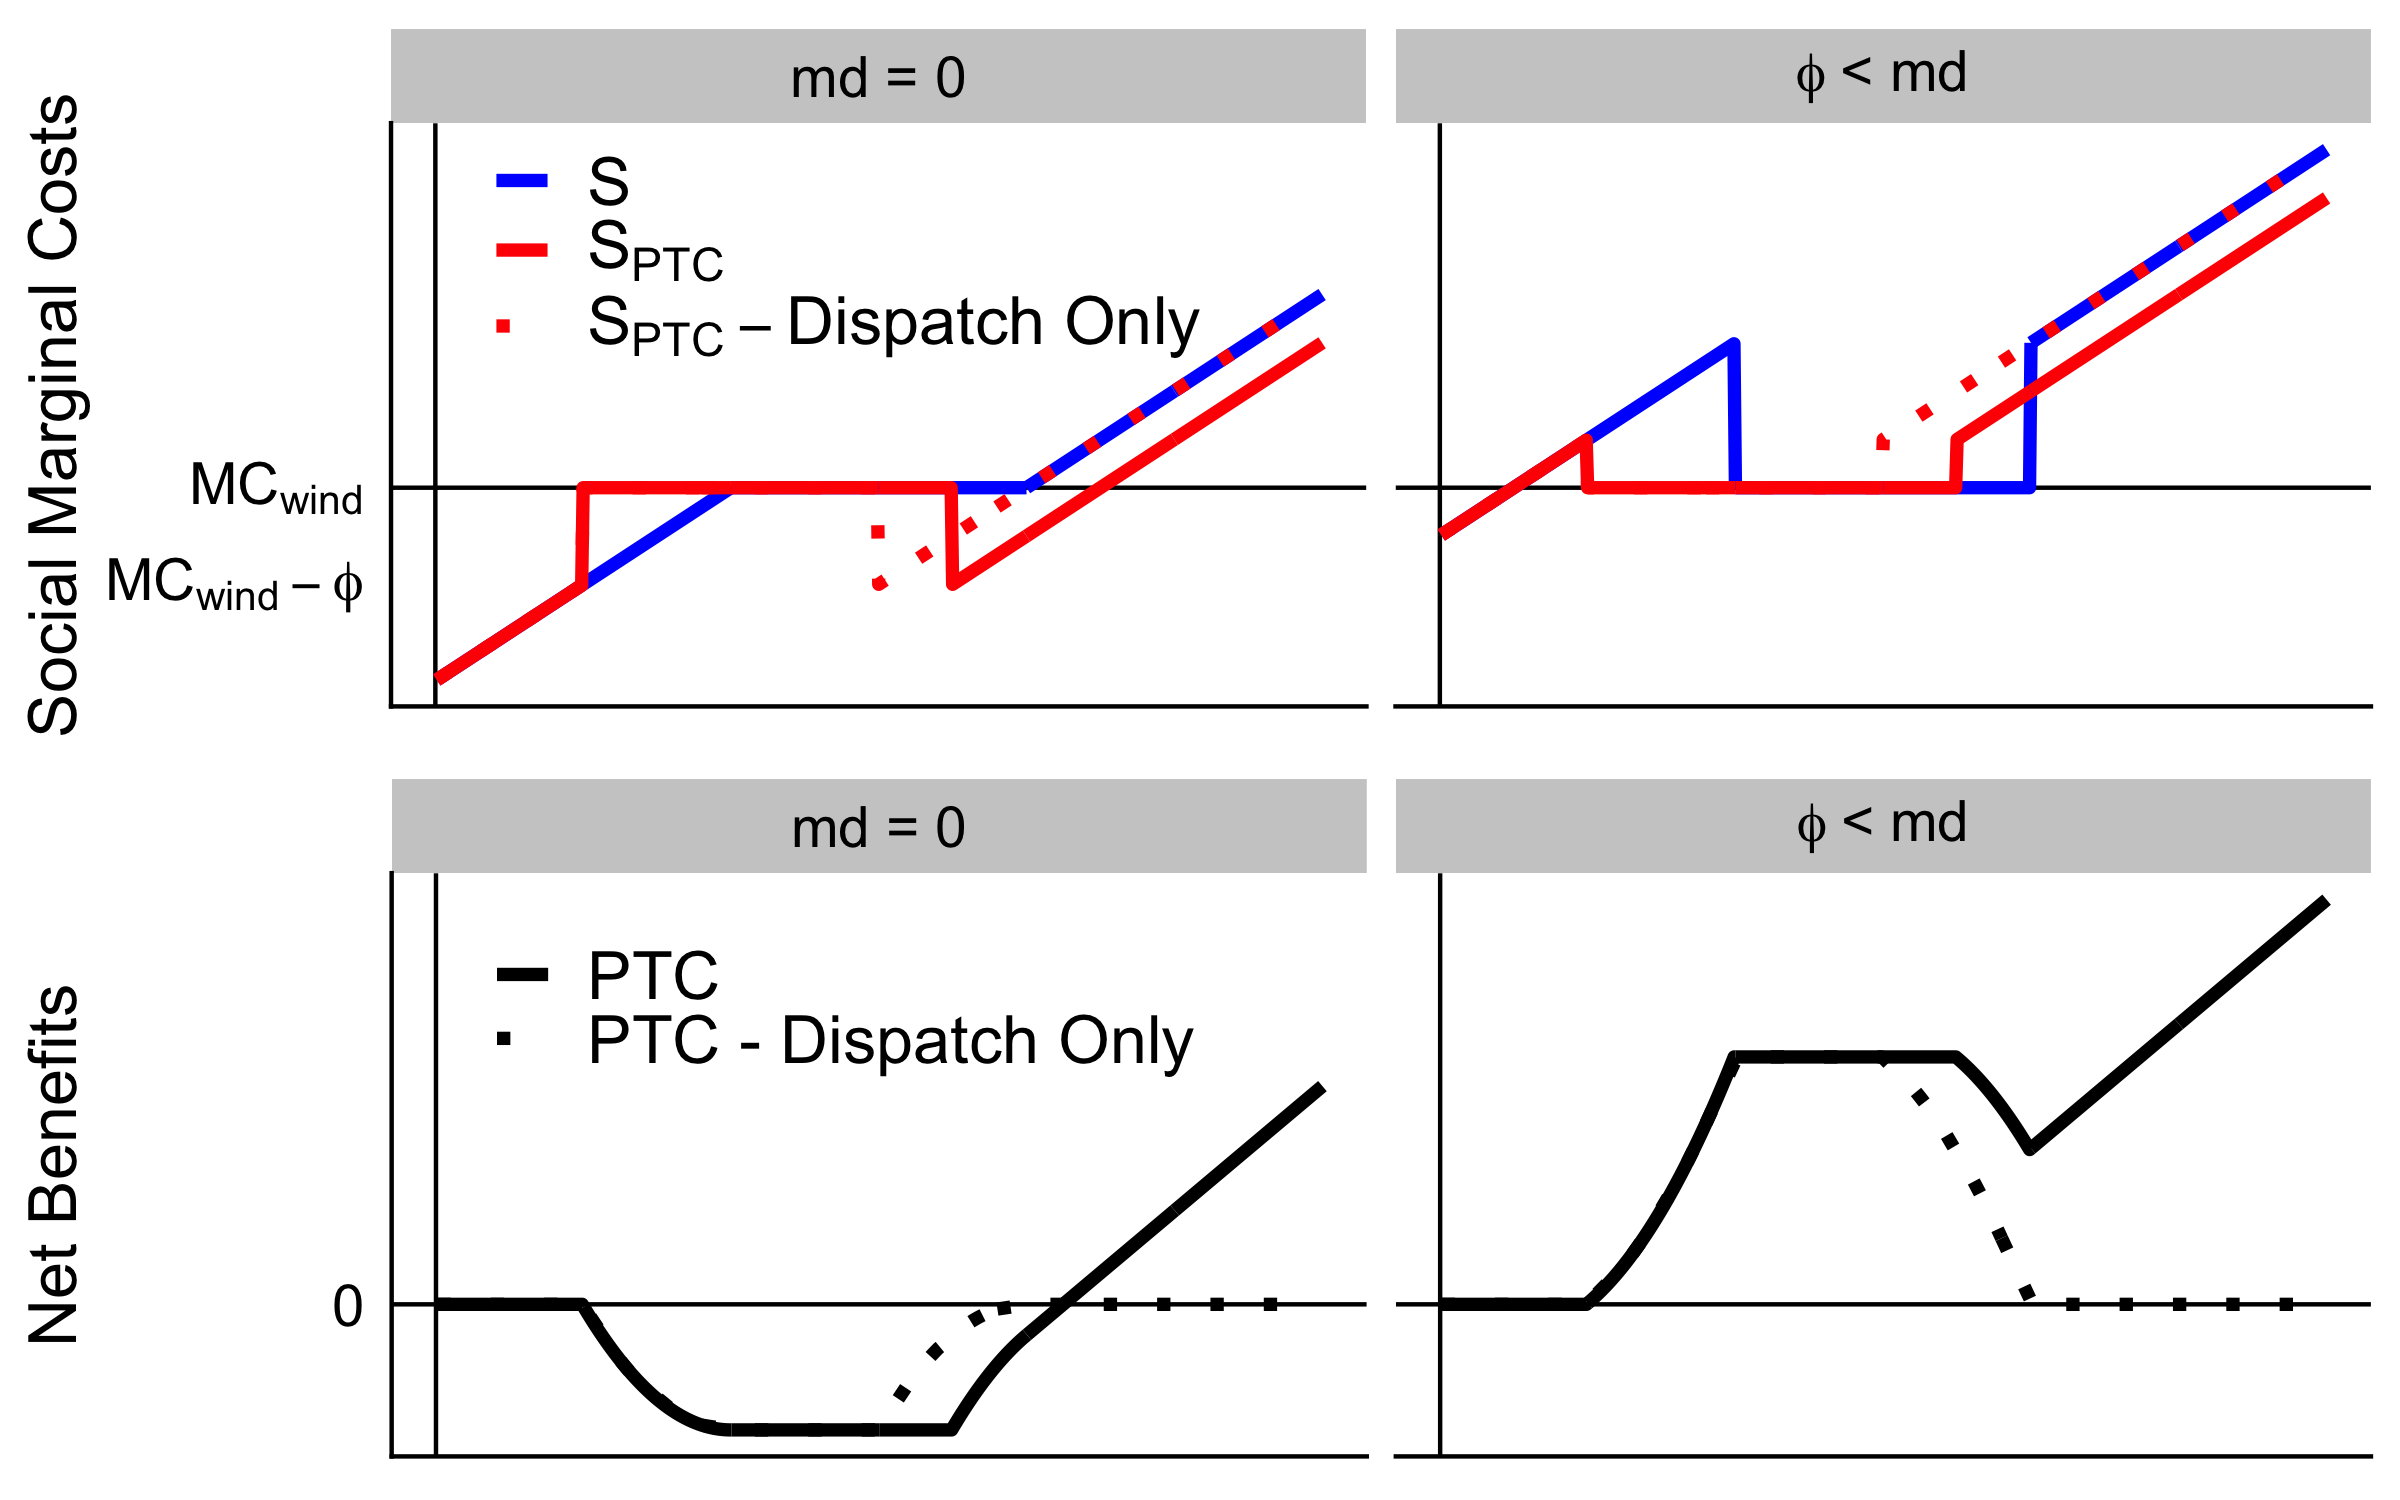
\includegraphics[width=0.85\linewidth]{net_benefits.png}
\end{center}
\end{figure}

The left column of Figure \ref{fig:mechanism_welfare} presents the case where there are no external marginal damages ($md$) associated with non-wind generation (for example, if wind displaces nuclear or hydro). Given that there are no unpriced externalities, the PTC generates welfare losses whenever wind is dispatched and cheaper resources are not. If the PTC increases availability, the net benefits are positive and increasing at high demand levels, because additional wind power displaces marginal plants with high production costs. The right column presents the opposite extreme, where the marginal damages from non-wind generation are larger than the subsidy.\footnote{If wind displaces coal-based power, then the avoided marginal damages from climate change alone would be about \$50/MWh -- double the PTC \citep{iawg_2016}.} If the PTC affects dispatch but not availability, any net benefits from the PTC come entirely during low demand hours. If the PTC also increases availability, net benefits continue to rise at high demand levels, always at a higher level than the $md=0$ case. Intermediate cases where $0 \le md \le \phi$ generate net benefits which lie between these extremes.\footnote{The short run marginal cost of wind generation is zero ($MC_{wind} = 0$). Thus, during the hours where the dispatch effect alone operates, prices will be negative under the PTC. While much has been made of the rise in the frequency of negative prices, and this has been attributed to the PTC, Figure \ref{fig:mechanism_welfare} makes it clear that there is nothing economically significant about $MC_{wind} = 0$. Even if $MC_{wind}$ were positive, the net benefits would be negative if $md = 0$. Conversely, net benefits can clearly be positive at $MC_{wind} = 0$ if $md > \phi$.}
% Avoided marginal damages of \$50 per MWh from coal is based on an SCC of $50/metric ton and emissions rate of 2.21 pounds per kWh

Several recent papers provide empirical estimates of marginal damages which suggest our second extreme case -- $\phi < md$  -- holds on average for most regions and time periods across the United States. For example, \citet{holland_are_2016} estimate average marginal damages and find that they are higher than the PTC in most regions and at almost all hours of the day (see appendix Figure \ref{fig:md_np_hmmy}). \citet{fell_emissions_2021} focus on the environmental benefits of wind electricity and find that annual average marginal damages avoided in MISO and ERCOT are higher than the PTC every hour of the day. As the preceding discussion makes clear, to the extent that the majority of our estimated output effect comes from the dispatch effect, then net benefits will hinge upon the marginal emission rates during very low demand periods. \citet{callaway_location_2018} estimate the marginal operating emission rates (MOERs) for six large ISOs. In Appendix~\ref{Appendix:NegativePrices} we show that these MOERs are generally highest during the hours of the day and seasons when demand is lowest. The most relevant empirical evidence comes from an econometric study of the marginal emissions impacts of wind power at different levels of demand in Texas, which, conveniently, is also the modal state in our sample. \citet{novan_valuing_2015} finds the marginal external benefits from wind are actually \emph{highest} during periods of low demand because they are most likely to offset non-wind generators that impose large external costs. Based on this evidence, we conclude that the increased wind output generated by the PTC likely increases net benefits \emph{on average} regardless of the mechanism. 

The preceding analysis has ignored the possibility that output subsidies could reduce the efficiency of scheduling, dispatching, and delivering power on the grid as a whole. \citet{petersen2021Spain} study the \emph{removal} of output subsidies for wind plants in Spain that were already in operation. They find that switching to capacity-based payments reduced system costs by avoiding inefficient dispatch on days with high wind. We do not consider the impact of the 1603 grant program on such balancing costs here, as the share of wind penetration in the United States during our sample is much smaller than in Spain. However, given ambitious state renewable energy goals in much of the United States, these considerations could be important for determining the second-best subsidy design in the future. 

\subsection{Extensive Margin Effects \label{subsec:Extensive}}

So far, we have focused on estimating how much more output 1603 recipients would have produced had they received the PTC, conditional on operating. In this section we consider whether the 1603 program had any effect on the number of plants we observe operating in the first place. This is important because, while our IV and matching estimators address concerns about selection \textit{between} subsidies, both strategies leverage the fact that plants that entered before 2009 did not have access to the 1603 program. If the 1603 grant encouraged more entry, and if these marginal plants were (unobservably) less productive, then extensive margin selection may confound our estimate of the intensive margin response to output subsidies. 

The abrupt introduction of the 1603 program, combined with its short duration relative to project lead times, make it highly unlikely that new wind projects would be conceived entirely in response to the output subsidy. However, at any given point in time, there are many potential projects in various stages of planning, some of which will never come to fruition, and the 1603 grant may have screened in a higher share of these potential projects than in previous years. To assess this, we look for evidence of a change in plant cancellations using the EIA's annual proposed plants list. Figure~\ref{fig:proposed_completed_on_time} presents the share of plants that are completed within one year of their original expected completion year, plotted by expected completion year. The policy period, 2009-2012, is shaded. The completion rates look very similar during the policy period and the years preceding it, and, importantly, the share of plants that are completed does not appear to increase in response to the investment subsidy.\footnote{We also graph the share of plants that are \textit{ever} completed by year of initial proposal in Appendix Figure~\ref{fig:proposed_ever_completed}. Completion rates remain similar before and during the policy period under this alternative metric. This graph also shows that the large drop in on-time completions in 2013 in Figure~\ref{fig:proposed_completed_on_time} indicates delay, not termination, of these post 1603 projects. When Congress extended the PTC for 2013, it made a major change to the eligibility for the tax credit: a wind farm had to begun construction in 2013 to be eligible for the tax credit for its first ten years of generation, in lieu of the previous requirement that a wind farm had to be placed into service.} It thus appears unlikely that productivity estimates will be confounded by low productivity plants being differentially screened in during the policy period. 

\begin{figure}[h]
\caption{Share of Plants Completed on Time, Plotted by Year of Initial Expected Completion\label{fig:proposed_completed_on_time}}
\vspace{-15pt}
\begin{center}
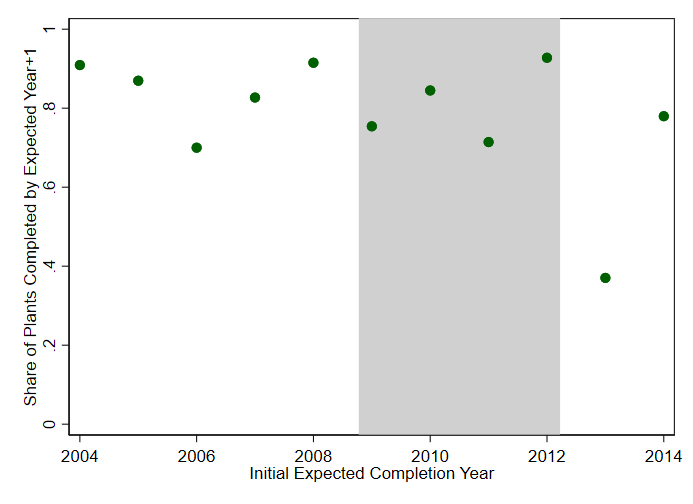
\includegraphics[width=0.75\linewidth]{proposal_data_completed_on_time.png}
\end{center}
\vspace{-15pt}
\footnotesize
The initial expected completion year is the year the generator was first scheduled to start operation. Completion is determined based on whether each plant entered into the EIA-860 operable data. Plots are based on the subset of plants that last appeared in the EIA-860 proposed data prior to 2016. Shading indicates the years during which new plants were eligible for the 1603 grant (2009 to 2012).
\end{figure}

We now consider whether the rate at which projects were completed from 2009 to 2012 would have been \emph{even lower} than previous years absent the 1603 grant program. This program was created in response to the concern that many projects already under development in late 2008 could be rendered unprofitable under the PTC by the widespread financial collapse, as discussed in Section \ref{subsec:RenewablePolicies}. Therefore, while we show that 1603-claiming plants produce less output than they would have under the PTC, we must weigh these inframarginal output losses against any extensive margin gains to compute the net aggregate effect of the program on wind output. Unfortunately, we are unable to estimate the extensive margin effect as rigorously as the intensive margin effect due to the small number of plants entering each period and the time series nature of the policy variation. In lieu of a formal entry model or tests for a time-series break, we instead perform a simple accounting calculation to identify ``marginal'' plants  -- i.e., power plants claiming the 1603 grant that appear profitable under the investment subsidy but not the PTC.\footnote{We describe this calculation briefly here and provide additional details in Appendix~\ref{Appendix:Profitability-calculation-detail}.}

For each 1603 recipient, we construct an estimate of discounted lifetime profits under the program:
\begin{equation}
\pi_i^{1603}=\sum_{t=1}^{t=25} \left(\frac{p_{it}}{(1+r)^{t}}\right) Q_{it} - \frac{c_{it}}{(1+r)^{t}} -(1-s)F_i\label{eq:pi1603} \quad
\end{equation}
Plant-specific output prices ($p_{it}$) are obtained from resale revenues reported on EIA Form 923 and power purchase agreements from AWEA and Bloomberg New Energy Finance (BNEF). We also include in $p_{it}$ estimated marginal revenue from the sale of RECs under state-level renewable portfolio standards using data from Marex Spectron and Lawrence Berkeley National Laboratory. Plants are assumed to remain in service for 25 years ($t$), and right censored prices and quantities are imputed with the observed (real) averages for each plant. Annual net revenue is obtained by subtracting operations and maintenance costs ($c_{it}$) of \$29/kW/year \citep{wiser_2018_2019}, and these flows are discounted at an assumed five percent real interest rate ($r$). Fixed investment costs ($F_i$) are obtained by dividing the observed 1603 grant award amount from Treasury by the fraction of investment costs covered by the program ($s=0.3$).

To compute ``counterfactual'' profits under the PTC we make two modifications to the discounted profit function:
\begin{equation}
\pi_i^{PTC}=\sum_{t=1}^{t=25}\left(\frac{p_{it}}{(1+r)^t} + \frac{\phi_{it}}{(1+r^{tax})^t} \right) Q_{it} 
 + \frac{\frac{1}{2} \phi_{it}}{(1+r^{tax})^t} \Delta Q_{it}(\phi_{it})
 - \frac{c_{it}}{(1+r)^t} - F_i\label{eq:piPTC}
\end{equation}
Under the PTC, firms forego the investment subsidy $s$, but gain $\phi$ additional dollars per unit output for the first ten years of operation. During this period, the PTC was equal to \$23 per MWh in tax credits. However, these tax credits need to monetized, and are thus less valuable than cash. In order to account for this additional cost of monetizing tax equity, we discount the PTC revenue streams by an assumed eight percent tax equity yield,\footnote{This approach to modeling the PTC differs conceptually from \cite{johnston_nonrefundable_2019}, who assumes that all revenue streams are discounted at the same rate, and estimates that firms appear to ``value'' PTC flow payments at 85 cents on the dollar. A 10 year annuity discounted at $r^{tax} = .08$ is worth 87\% of the same payment stream discounted at $r=.05$. Thus, using the observed tax equity yield to discount PTC payments generates essentially the same implicit valuation.} which is the modal value of the tax equity yield over 2009-2012 presented in \citet{bolinger_analysis_2014}.\footnote{Modeling how changes in firms' subsidy choices might affect equilibrium tax equity yields is beyond the scope of this paper. However, we present sensitivity analysis using the maximum observed yield of 10.5 percent in Appendix \ref{Appendix:1603eval}.} To capture this, we modify equation \ref{eq:pi1603} by adding $\phi_{it} / (1+r^{tax})^t$ to firms' marginal revenues for their inframarginal output, $Q_{it}$, and replacing $(1-s)F_i$ with $F_i$. 

The second modification we make to equation \ref{eq:pi1603} is that we account for firms' endogenous output responses estimated in Section \ref{sec:Empirical-Strategy}. We denote this increase in output under the PTC by $\Delta Q_{it}(\phi_{it})$. We compute $\Delta Q_{it}(\phi_{it})$ by increasing the observed capacity factor for each plant by $3.3$ percentage points (reflecting the average of our preferred IV and matching results) for the first ten years of operation. The revenues and costs associated with this marginal output may be different from the estimates we use for inframarginal output.\footnote{For example, prices may be lower if some of the electricity is sold at zero or negative prices. Increasing output may be costly.} To be conservative, we assume that net marginal revenues for this marginal output are half the PTC subsidy value. This is equivalent to assuming linear marginal costs for producing this marginal output, starting at \textit{whatever} price is received for marginal output and increasing by $\phi$.

\begin{figure}[h] 
\begin{center}
\caption{PTC Profits vs 1603 Profits for 1603 Recipients \label{fig:1603_vs_PTC_scatter}}
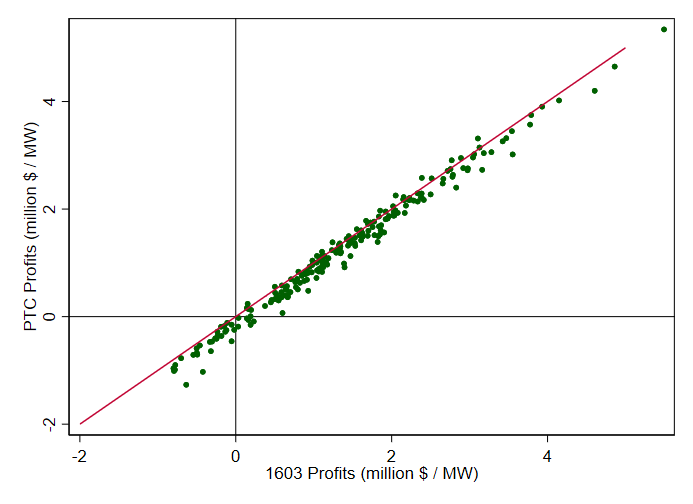
\includegraphics[width=0.75\linewidth]{1603_vs_PTC_pi_scatter.png}
\end{center}
\end{figure}

Figure~\ref{fig:1603_vs_PTC_scatter} presents a scatter plot of these two profit measures for plants selecting the 1603 grant. The 45-degree line reflects parity between the two, and, unsurprisingly, most plants selecting the investment subsidy earn less money under the output subsidy. Despite this, the graph also makes clear that the difference in profitability across plants within subsidy type is an order of magnitude larger than the difference across subsidies within a plant. And, since the distribution of plants is not particularly dense near the origin, very few plants appear marginal to the 1603 grant program. Of the 211 \unskip 1603 recipients included in this figure, only 6 \unskip lie in the lower right quadrant, where expected 1603 profits are positive and expected PTC profits are negative.\footnote{This sample differs slightly from the sample used in Section \ref{sec:Empirical-Strategy} because we exclude plants with no price data and include plants who were omitted from the regression analysis due to missing wind speed data.} 

Estimating the full effect of the 1603 program on output requires taking a stand on the counterfactual entry status of the twenty-nine \unskip plants in the lower left quadrant, which do not appear profitable under either subsidy. One possibility is to assume that these plants are in fact marginal, and would not have entered without the 1603 grant program. Under this assumption, the 1603 program increased lifetime wind production by 85 \unskip million MWh, or 14 \unskip percent. In our view, this assumption is unlikely, given the graphical evidence on entry rates presented in Figure~\ref{fig:proposed_completed_on_time}. Instead, it seems more plausible that the apparent lack of profitability for these plants implies a policy-invariant unobservable (possibly in expectation) that would have encouraged these wind farms to enter with or without the 1603 grant.\footnote{There are many potential reasons why plants may appear unprofitable using this approach. We only observe a handful of years of output data, so our approach could understate the profits of wind farms that had low output realizations during the years we observe. We may have also underestimated state and local subsidies or overestimated O\&M costs and discount rates for some plants. However, even if we had perfectly accounted for all of these factors, it is likely that some plants that appeared profitable \emph{ex ante} will be unprofitable \emph{ex post} due to low price and wind realizations.} Under this assumption, the 1603 grant program \textit{reduced} production by 25million MWh, relative to a scenario in which all plants had received the PTC. Additional results and sensitivity analysis are presented in Appendix \ref{Appendix:1603eval}.

\subsection{Cost-Effectiveness \label{sec:costEffectiveness}}

The previous section estimated the impact of the 1603 grant program on wind output and entry. On net, these changes imply that the 1603 grant program increased the federal cost per unit of wind energy by 7 \unskip to 8 \unskip percent, compared to the PTC status quo.\footnote{See Appendix \ref{Appendix:CostEffectiveness-calculation-detail} for the details of the calculation.} While this is useful for evaluating the 1603 program, several details limit any generalization of that result to the broader question of investment versus output subsidies.  First, there are idiosyncratic tax code differences between the two policies. The PTC was implemented as a tax credit, which was more difficult to monetize, while accepting the 1603 grant precluded some accelerated depreciation \citep{johnston_nonrefundable_2019}. Second, wind farm developers were able to select between subsidy options, which, given the zero sum nature of the transfer, \emph{must} raise the public cost for some plants. Finally, given the significant heterogeneity in wind quality across locations, the marginal public cost likely varies across different aggregate output targets. In this section, we ask whether investment or output subsidies are more cost-effective over a wide range of output targets, and absent any differential tax treatment. 

To gain intuition, we begin by considering the case where each plant's electricity production is invariant to the subsidy margin, conditional on the plant operating. Under this assumption, the insight of \citet{parish_relative_1982} is that we can determine whether investment subsidies will be cheaper than output subsidies by simply asking whether investment is used more intensively, or less productively, at the margin than on average. To investigate this, we use a simplified version of the firm profit function under an investment subsidy $s$ from equation \ref{eq:pi1603}, 
\begin{equation*}
\pi_i = p_i \bar{Q_i} - (1-s)F_i ,
\end{equation*}
where $\bar{Q_i}$ denotes the present discounted quantity of electricity produced, and $p_i$ is the price plant $i$ receives for its output. This can be rearranged to define the break-even investment subsidy for each plant,

\begin{equation}
  s^*_i = 1 - p_i \left( \frac{\bar{Q_i}}{F_i} \right) . \label{eq:BE_subsidy}
\end{equation}
Arranging plants in ascending order by break-even subsidy traces out a public investment subsidy supply curve. If all plants receive the same output price $p$, it is clear that $s^*_i$ is decreasing in investment productivity ($\bar{Q_i} / F_i$). In other words, at every subsidy level, the marginal plant will produce less electricity per dollar of investment than inframarginal plants will. Since investment subsidies operate at the margin, but pay out on average, and since output subsidies by definition pay the same subsidy per unit of output at the margin and on average, this means that an investment subsidy will be more cost-effective than an output subsidy. 

If we relax the assumptions of constant price and fixed output, the situation becomes less clear. In equation \ref{eq:BE_subsidy}, $s^*$ could be \emph{increasing} in investment productivity if output price and investment productivity were negatively correlated. It turns out that these two variables are in fact negatively correlated in the U.S. wind industry. Figure \ref{fig:price_vs_capprod_1603} presents a scatter plot of average output price and investment productivity for plants receiving the 1603 grant. The correlation between these measures is -.41\unskip. Thus, the relative cost-effectiveness of investment versus output subsidies in this setting is an empirical question. 

\begin{figure}[htbp] 
  \begin{center}
  \caption{Electricity Prices and Investment Productivities for 1603 Recipients \label{fig:price_vs_capprod_1603}}
  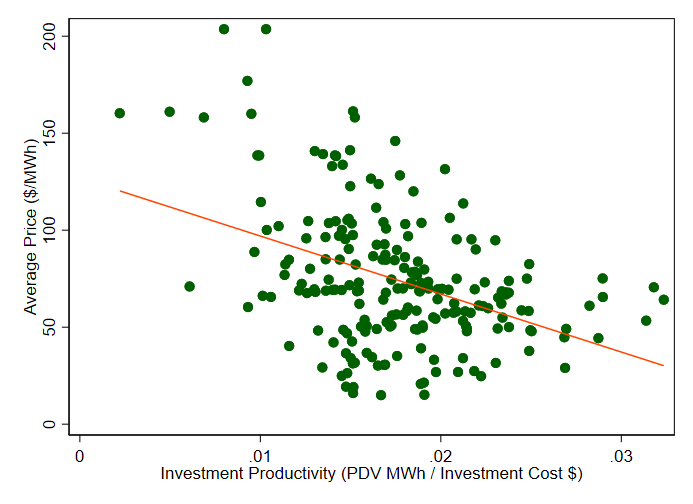
\includegraphics[width=0.75\linewidth]{price_vs_capprod_1603.png}
  \end{center}
  \vspace{-15pt}
  \footnotesize
  Each point is a plant. Investment productivity, on the x-axis, is the inverse of the levelized cost of electricity.
\end{figure}

We employ the accounting-based framework from the previous section to calculate the net effect of these forces while maintaining the assumption that plant output is fixed. Starting with the no subsidy case, we determine the number of profitable entrants. We then incrementally increase subsidies up to the observed level of the 1603 and PTC subsidies, $s=0.3$ and $\phi=\$23$ per MWh. For each subsidy level, we compute total discounted output, government expenditures, and the public levelized cost of energy (LCOE) for plants that are profitable at that subsidy level. This allows a direct comparison of the alternative subsidies: to minimize the public expenditure needed to reach a certain quantity of output, the government can choose whichever subsidy achieves that level of output at lower public LCOE.

Figure \ref{fig:pub_lcoe} presents the public cost per MWh of wind by subsidy type. Panel (a) restricts the analysis to plants that selected the 1603 grant, as in the previous section. We first compare the output subsidy with no output response (``Output - Fixed Q'') to the investment subsidy (``Investment''). By and large, these two subsidies appear similarly cost effective. This means that, for this sample, the negative correlation between output price and investment productivity is enough to offset the direct effect of investment productivity on cost-effectiveness when holding price fixed. In panel (b), we consider the cost-effectiveness of investment and output subsidies for all the plants in our sample.\footnote{Estimating profits for PTC recipients is complicated by the fact that the government does not track investment costs for these firms. We compile cost information from a variety of sources, including SNL Energy, Bloomberg New Energy Finance (BNEF), state tax filings, regulatory filings and press releases. For the remaining plants, we predict missing costs using regression. Additional details provided in Appendix \ref{Appendix:CostEffectiveness-calculation-detail}.} In this larger sample, the public LCOE of output subsidies in the fixed quantity case are substantially lower than investment subsidies at most points in the supply curve. This is because the negative correlation between output prices and investment productivity is even stronger in the full sample, at -.51\unskip.\footnote{In appendix \ref{Appendix:PriceCorrelation} we provide an alternative illustration of this point. We recompute the public LCOE of output and investment subsidies under a scenario where we assume that all firms receive the same output price. Figure \ref{fig:pub_lcoe_meanprice} shows that, under this scenario, output subsidies are uniformly more expensive than investment subsidies when output is held fixed. The two are comparable when production is allowed to respond to output incentives.}

\begin{figure}[htb]
  \caption{Public LCOE vs Electricity Generation by Subsidy Type \label{fig:pub_lcoe}}
  \begin{center}%\centering
  \begin{subfigure}[b]{0.495\textwidth}
    \caption{1603 Recipients \label{fig:pub_lcoe_1603}}
    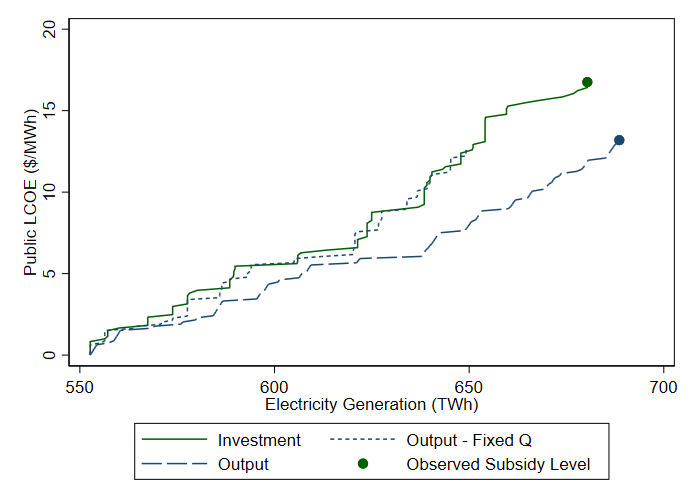
\includegraphics[width=\textwidth]{plcoe_plot_1603plants.png}
  \end{subfigure} \hfill
  \begin{subfigure}[b]{0.495\textwidth}
    \caption{All Plants \label{fig:pub_lcoe_all}}
    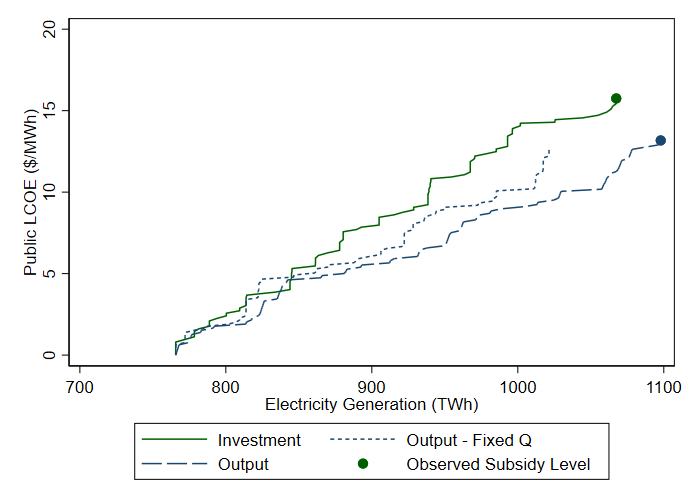
\includegraphics[width=\textwidth]{plcoe_plot_all.png}
  \end{subfigure}
  \end{center}
  \vspace{-15pt}
  \footnotesize
  Each line plots the average public subsidy per unit of wind generation (LCOE) as a function of the total amount of wind generation subsidized. These are constructed by gradually increasing the subsidy from zero to the observed subsidy rates of the 1603 grant (investment) and PTC (output) subsidies. For output subsidy levels inframarginal to the PTC, we scale the estimated impact of the PTC on production linearly. For comparison, the ``Output - Fixed Q'' line plots the LCOE under the assumption that output is subsidized, but that this increase in marginal incentives does not affect plant productivity, conditional on operating. Panel (a) restricts the set of potential entrants to those selecting the 1603 grant, while panel (b) includes all wind farms entering between 2009 and 2012. In both figures, plants which are not marginal to either subsidy over the relevant range are assumed to always enter. The total output of these plants is reflected in the X-intercept of each figure. 
\end{figure}

If output responds to marginal production incentives, as we found in Section \ref{sec:Empirical-Strategy}, the public cost savings relative to investment subsidies become even larger. There are two channels for this. First, if plants produce more under output subsidies, they will earn some additional profit from this additional quantity. This means that the break-even output subsidy for each plant will be slightly lower, shifting the ``Fixed Q'' supply curve down at each quantity level. Second, if firms increase production in response to marginal incentives, \emph{inframarginal} plants will increase production as the break-even subsidy of the marginal recipient increases. This shifts the supply curve to the right at each subsidy level. In order to incorporate this response, we need to estimate the output firms would have produced at different levels of the output subsidy. Since the level of the PTC does not vary in our sample, it is not possible to directly estimate how output varies with the subsidy level. Instead, to approximate output under intermediate levels of the output subsidy, we scale our estimated output effect linearly. For example, the effect of an output subsidy of \$11.50 per MWh, half the value of the PTC, would be half our estimated output effect. As a result, changing the level of the subsidy affects plant profitability through both the level of the subsidy and the quantity of output.
 
Once we account for how output responds to the output subsidy, output subsidies (labeled ``Output'' in Figure \ref{fig:pub_lcoe}) appear clearly preferable to investment subsidies in both samples.\footnote{Figure \ref{fig:pub_lcoe} summarizes the results under our baseline assumptions. If firms' profits on production marginal to the output subsidy were less than half the output subsidy, or if the output effect scaled less than linearly, the results would lie between ``Output'' and ``Output - Fixed Q.''} In the 1603 plant sample, an output subsidy of $\phi = \$ 20.7$/MWh results in the same total quantity of wind power as the 1603 investment subsidy rate of $s=0.3$. At this level, the public LCOEs are $\$ 16.76$/MWh and $\$ 11.82$/MWh, for a $29$ percent reduction in cost per MWh under the PTC.\footnote{Note that these public LCOEs are lower than Table \ref{tab:policyeval}, which includes accelerated depreciation.} In the full sample of plants entering from 2009 to 2012, an output subsidy of $\phi = \$ 19.78$/MWh results in the same total quantity of wind power as the 1603 investment subsidy rate of $s=0.3$. At this level, the public LCOEs are $\$ 15.75$/MWh and $\$ 11.26$/MWh, which is also a $29$ percent reduction.

\section{Conclusion \label{sec:Conclusion}}

The economically efficient response to the problem of pollution externalities from energy generation is to impose a Pigouvian tax on emissions, not to subsidize emissions-free production. Nevertheless, the use of both investment and output subsidies for green energy is widespread. For example, in the United States, the Federal government subsidizes solar energy through the Investment Tax Credit. At the same time, 33 states offer residential solar adopters some form of ``performance-based incentive'' (PBI), which pays above private marginal value for each unit of solar output.\footnote{Source: \href{https://www.solarpowerrocks.com/affordable-solar/what-are-solar-performance-payments-srec-pbi/}{https://www.solarpowerrocks.com/affordable-solar/what-are-solar-performance-payments-srec-pbi/}, accessed 7/10/2019. These take the form of feed-in tariffs, performance premiums, and solar renewable energy certificates.} In the European Union, 21 countries subsidized qualifying renewables using feed-in tariffs (payments per unit energy delivered to the grid), while seven offered investment grants or tax credits \citep{JENNER2013385}. 

In this paper, we exploit a natural experiment to directly estimate the relative cost-effectiveness of using output versus investment subsidies to promote wind energy. We find that by reducing output incentives on the margin, the Section 1603 grant program caused wind farms to generate 10 \unskip to 12percent less power than they would have under the PTC. Using firm-specific data on production, output prices, and investment costs, we find that very few plants appear profitable under one subsidy type but not the other. After standardizing the tax treatment of these subsidies and accounting for extensive margin effects, we show that output subsidies are more cost-effective over a large range of output targets. 

What are the lessons for subsidies outside of energy policy? Investment subsidies are observed in several important settings where the social benefits of investment appear to be tied to output, such as affordable housing and research and development. The relative cost-effectiveness of output subsidies in these settings will depend on the production primitives of those markets, and we make no claim that our results are informative about optimal targeting in those domains. Nevertheless, the fact that investment subsidies appear poorly targeted in this setting should motivate future empirical work in other settings.

\pagebreak
%\begin{singlespace}
%\bibliographystyle{mychicago}
\bibliographystyle{jaere}
\bibliography{1603_all}
%\end{singlespace}

\end{document}
